% Auto-generated by cmd/render — the contrast map as a TikZ figure.
% One grid per Kind over the scored scenarios. Orange = signal (verdict
% from fdr.gen.tex), grey = measured, no marginal signal (deeper grey =
% higher raw saliency, i.e. destabilization), dashed outline = negative
% control (defines the fragility floor), dark cell with * = deciding locus
% (the injected fault, never scored).
% \input-able fragment; requires \usepackage{tikz}.

\par\medskip\noindent{\small\bfseries ClusterRole}\par\smallskip
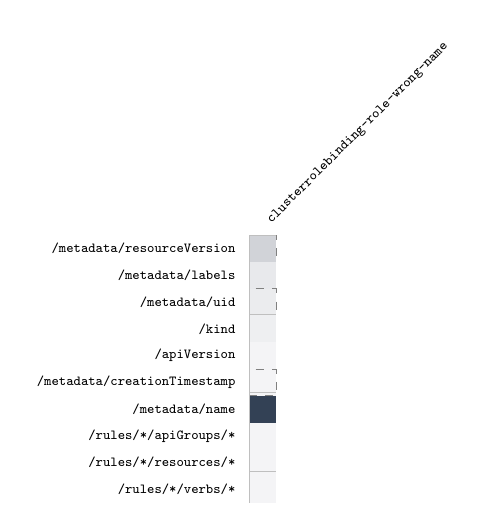
\begin{tikzpicture}[x=3.4mm,y=3.4mm]
\node[rotate=45,anchor=west,font=\ttfamily\tiny] at (0.5,0.25) {clusterrolebinding-role-wrong-name};
\node[anchor=east,font=\ttfamily\tiny] at (-0.15,-0.5) {/metadata/resourceVersion};
\fill[fill={rgb,255:red,209;green,211;blue,216}] (0,-1) rectangle ++(1,1);
\draw[gray,dashed,line width=0.2pt] (0,-1) rectangle ++(1,1);
\node[anchor=east,font=\ttfamily\tiny] at (-0.15,-1.5) {/metadata/labels};
\fill[fill={rgb,255:red,232;green,233;blue,236}] (0,-2) rectangle ++(1,1);
\node[anchor=east,font=\ttfamily\tiny] at (-0.15,-2.5) {/metadata/uid};
\fill[fill={rgb,255:red,235;green,236;blue,238}] (0,-3) rectangle ++(1,1);
\draw[gray,dashed,line width=0.2pt] (0,-3) rectangle ++(1,1);
\node[anchor=east,font=\ttfamily\tiny] at (-0.15,-3.5) {/kind};
\fill[fill={rgb,255:red,238;green,239;blue,241}] (0,-4) rectangle ++(1,1);
\node[anchor=east,font=\ttfamily\tiny] at (-0.15,-4.5) {/apiVersion};
\fill[fill={rgb,255:red,244;green,244;blue,246}] (0,-5) rectangle ++(1,1);
\node[anchor=east,font=\ttfamily\tiny] at (-0.15,-5.5) {/metadata/creationTimestamp};
\fill[fill={rgb,255:red,244;green,244;blue,246}] (0,-6) rectangle ++(1,1);
\draw[gray,dashed,line width=0.2pt] (0,-6) rectangle ++(1,1);
\node[anchor=east,font=\ttfamily\tiny] at (-0.15,-6.5) {/metadata/name};
\fill[fill={rgb,255:red,51;green,65;blue,85}] (0,-7) rectangle ++(1,1);
\node[white,font=\tiny] at (0.5,-7.5) {$\ast$};
\node[anchor=east,font=\ttfamily\tiny] at (-0.15,-7.5) {/rules/*/apiGroups/*};
\fill[fill={rgb,255:red,244;green,244;blue,246}] (0,-8) rectangle ++(1,1);
\node[anchor=east,font=\ttfamily\tiny] at (-0.15,-8.5) {/rules/*/resources/*};
\fill[fill={rgb,255:red,244;green,244;blue,246}] (0,-9) rectangle ++(1,1);
\node[anchor=east,font=\ttfamily\tiny] at (-0.15,-9.5) {/rules/*/verbs/*};
\fill[fill={rgb,255:red,244;green,244;blue,246}] (0,-10) rectangle ++(1,1);
\draw[gray!50,line width=0.2pt] (0,0) grid (1,-10);
\end{tikzpicture}

\par\medskip\noindent{\small\bfseries ServiceAccount}\par\smallskip
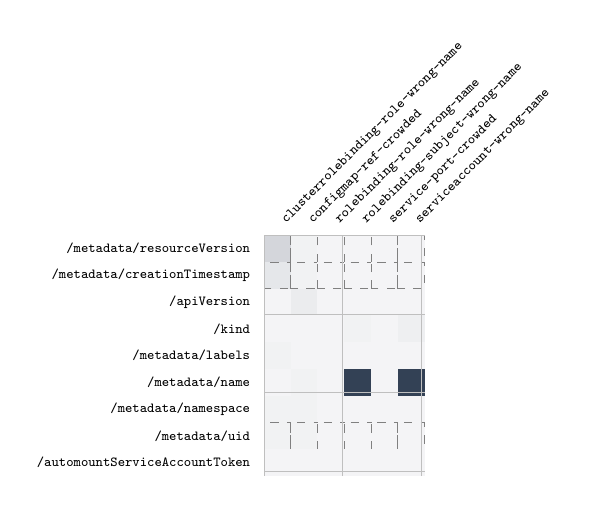
\begin{tikzpicture}[x=3.4mm,y=3.4mm]
\node[rotate=45,anchor=west,font=\ttfamily\tiny] at (0.5,0.25) {clusterrolebinding-role-wrong-name};
\node[rotate=45,anchor=west,font=\ttfamily\tiny] at (1.5,0.25) {configmap-ref-crowded};
\node[rotate=45,anchor=west,font=\ttfamily\tiny] at (2.5,0.25) {rolebinding-role-wrong-name};
\node[rotate=45,anchor=west,font=\ttfamily\tiny] at (3.5,0.25) {rolebinding-subject-wrong-name};
\node[rotate=45,anchor=west,font=\ttfamily\tiny] at (4.5,0.25) {service-port-crowded};
\node[rotate=45,anchor=west,font=\ttfamily\tiny] at (5.5,0.25) {serviceaccount-wrong-name};
\node[anchor=east,font=\ttfamily\tiny] at (-0.15,-0.5) {/metadata/resourceVersion};
\fill[fill={rgb,255:red,212;green,214;blue,219}] (0,-1) rectangle ++(1,1);
\draw[gray,dashed,line width=0.2pt] (0,-1) rectangle ++(1,1);
\fill[fill={rgb,255:red,241;green,242;blue,243}] (1,-1) rectangle ++(1,1);
\draw[gray,dashed,line width=0.2pt] (1,-1) rectangle ++(1,1);
\fill[fill={rgb,255:red,244;green,244;blue,246}] (2,-1) rectangle ++(1,1);
\draw[gray,dashed,line width=0.2pt] (2,-1) rectangle ++(1,1);
\fill[fill={rgb,255:red,244;green,244;blue,246}] (3,-1) rectangle ++(1,1);
\draw[gray,dashed,line width=0.2pt] (3,-1) rectangle ++(1,1);
\fill[fill={rgb,255:red,244;green,244;blue,246}] (4,-1) rectangle ++(1,1);
\draw[gray,dashed,line width=0.2pt] (4,-1) rectangle ++(1,1);
\fill[fill={rgb,255:red,244;green,244;blue,246}] (5,-1) rectangle ++(1,1);
\draw[gray,dashed,line width=0.2pt] (5,-1) rectangle ++(1,1);
\node[anchor=east,font=\ttfamily\tiny] at (-0.15,-1.5) {/metadata/creationTimestamp};
\fill[fill={rgb,255:red,229;green,231;blue,234}] (0,-2) rectangle ++(1,1);
\draw[gray,dashed,line width=0.2pt] (0,-2) rectangle ++(1,1);
\fill[fill={rgb,255:red,241;green,242;blue,243}] (1,-2) rectangle ++(1,1);
\draw[gray,dashed,line width=0.2pt] (1,-2) rectangle ++(1,1);
\fill[fill={rgb,255:red,244;green,244;blue,246}] (2,-2) rectangle ++(1,1);
\draw[gray,dashed,line width=0.2pt] (2,-2) rectangle ++(1,1);
\fill[fill={rgb,255:red,244;green,244;blue,246}] (3,-2) rectangle ++(1,1);
\draw[gray,dashed,line width=0.2pt] (3,-2) rectangle ++(1,1);
\fill[fill={rgb,255:red,244;green,244;blue,246}] (4,-2) rectangle ++(1,1);
\draw[gray,dashed,line width=0.2pt] (4,-2) rectangle ++(1,1);
\fill[fill={rgb,255:red,244;green,244;blue,246}] (5,-2) rectangle ++(1,1);
\draw[gray,dashed,line width=0.2pt] (5,-2) rectangle ++(1,1);
\node[anchor=east,font=\ttfamily\tiny] at (-0.15,-2.5) {/apiVersion};
\fill[fill={rgb,255:red,244;green,244;blue,246}] (0,-3) rectangle ++(1,1);
\fill[fill={rgb,255:red,235;green,236;blue,238}] (1,-3) rectangle ++(1,1);
\fill[fill={rgb,255:red,244;green,244;blue,246}] (2,-3) rectangle ++(1,1);
\fill[fill={rgb,255:red,244;green,244;blue,246}] (3,-3) rectangle ++(1,1);
\fill[fill={rgb,255:red,244;green,244;blue,246}] (4,-3) rectangle ++(1,1);
\fill[fill={rgb,255:red,244;green,244;blue,246}] (5,-3) rectangle ++(1,1);
\node[anchor=east,font=\ttfamily\tiny] at (-0.15,-3.5) {/kind};
\fill[fill={rgb,255:red,244;green,244;blue,246}] (0,-4) rectangle ++(1,1);
\fill[fill={rgb,255:red,244;green,244;blue,246}] (1,-4) rectangle ++(1,1);
\fill[fill={rgb,255:red,244;green,244;blue,246}] (2,-4) rectangle ++(1,1);
\fill[fill={rgb,255:red,241;green,242;blue,243}] (3,-4) rectangle ++(1,1);
\fill[fill={rgb,255:red,244;green,244;blue,246}] (4,-4) rectangle ++(1,1);
\fill[fill={rgb,255:red,238;green,239;blue,241}] (5,-4) rectangle ++(1,1);
\node[anchor=east,font=\ttfamily\tiny] at (-0.15,-4.5) {/metadata/labels};
\fill[fill={rgb,255:red,241;green,242;blue,243}] (0,-5) rectangle ++(1,1);
\fill[fill={rgb,255:red,244;green,244;blue,246}] (1,-5) rectangle ++(1,1);
\fill[fill={rgb,255:red,244;green,244;blue,246}] (2,-5) rectangle ++(1,1);
\fill[fill={rgb,255:red,244;green,244;blue,246}] (3,-5) rectangle ++(1,1);
\fill[fill={rgb,255:red,244;green,244;blue,246}] (4,-5) rectangle ++(1,1);
\fill[fill={rgb,255:red,244;green,244;blue,246}] (5,-5) rectangle ++(1,1);
\node[anchor=east,font=\ttfamily\tiny] at (-0.15,-5.5) {/metadata/name};
\fill[fill={rgb,255:red,244;green,244;blue,246}] (0,-6) rectangle ++(1,1);
\fill[fill={rgb,255:red,241;green,242;blue,243}] (1,-6) rectangle ++(1,1);
\fill[fill={rgb,255:red,244;green,244;blue,246}] (2,-6) rectangle ++(1,1);
\fill[fill={rgb,255:red,51;green,65;blue,85}] (3,-6) rectangle ++(1,1);
\node[white,font=\tiny] at (3.5,-6.5) {$\ast$};
\fill[fill={rgb,255:red,244;green,244;blue,246}] (4,-6) rectangle ++(1,1);
\fill[fill={rgb,255:red,51;green,65;blue,85}] (5,-6) rectangle ++(1,1);
\node[white,font=\tiny] at (5.5,-6.5) {$\ast$};
\node[anchor=east,font=\ttfamily\tiny] at (-0.15,-6.5) {/metadata/namespace};
\fill[fill={rgb,255:red,241;green,242;blue,243}] (0,-7) rectangle ++(1,1);
\fill[fill={rgb,255:red,241;green,242;blue,243}] (1,-7) rectangle ++(1,1);
\fill[fill={rgb,255:red,244;green,244;blue,246}] (2,-7) rectangle ++(1,1);
\fill[fill={rgb,255:red,244;green,244;blue,246}] (3,-7) rectangle ++(1,1);
\fill[fill={rgb,255:red,244;green,244;blue,246}] (4,-7) rectangle ++(1,1);
\fill[fill={rgb,255:red,244;green,244;blue,246}] (5,-7) rectangle ++(1,1);
\node[anchor=east,font=\ttfamily\tiny] at (-0.15,-7.5) {/metadata/uid};
\fill[fill={rgb,255:red,241;green,242;blue,243}] (0,-8) rectangle ++(1,1);
\draw[gray,dashed,line width=0.2pt] (0,-8) rectangle ++(1,1);
\fill[fill={rgb,255:red,241;green,242;blue,243}] (1,-8) rectangle ++(1,1);
\draw[gray,dashed,line width=0.2pt] (1,-8) rectangle ++(1,1);
\fill[fill={rgb,255:red,244;green,244;blue,246}] (2,-8) rectangle ++(1,1);
\draw[gray,dashed,line width=0.2pt] (2,-8) rectangle ++(1,1);
\fill[fill={rgb,255:red,244;green,244;blue,246}] (3,-8) rectangle ++(1,1);
\draw[gray,dashed,line width=0.2pt] (3,-8) rectangle ++(1,1);
\fill[fill={rgb,255:red,244;green,244;blue,246}] (4,-8) rectangle ++(1,1);
\draw[gray,dashed,line width=0.2pt] (4,-8) rectangle ++(1,1);
\fill[fill={rgb,255:red,244;green,244;blue,246}] (5,-8) rectangle ++(1,1);
\draw[gray,dashed,line width=0.2pt] (5,-8) rectangle ++(1,1);
\node[anchor=east,font=\ttfamily\tiny] at (-0.15,-8.5) {/automountServiceAccountToken};
\fill[fill={rgb,255:red,244;green,244;blue,246}] (0,-9) rectangle ++(1,1);
\fill[fill={rgb,255:red,244;green,244;blue,246}] (1,-9) rectangle ++(1,1);
\fill[fill={rgb,255:red,244;green,244;blue,246}] (2,-9) rectangle ++(1,1);
\fill[fill={rgb,255:red,244;green,244;blue,246}] (3,-9) rectangle ++(1,1);
\fill[fill={rgb,255:red,244;green,244;blue,246}] (4,-9) rectangle ++(1,1);
\fill[fill={rgb,255:red,244;green,244;blue,246}] (5,-9) rectangle ++(1,1);
\draw[gray!50,line width=0.2pt] (0,0) grid (6,-9);
\end{tikzpicture}

\par\medskip\noindent{\small\bfseries Service}\par\smallskip
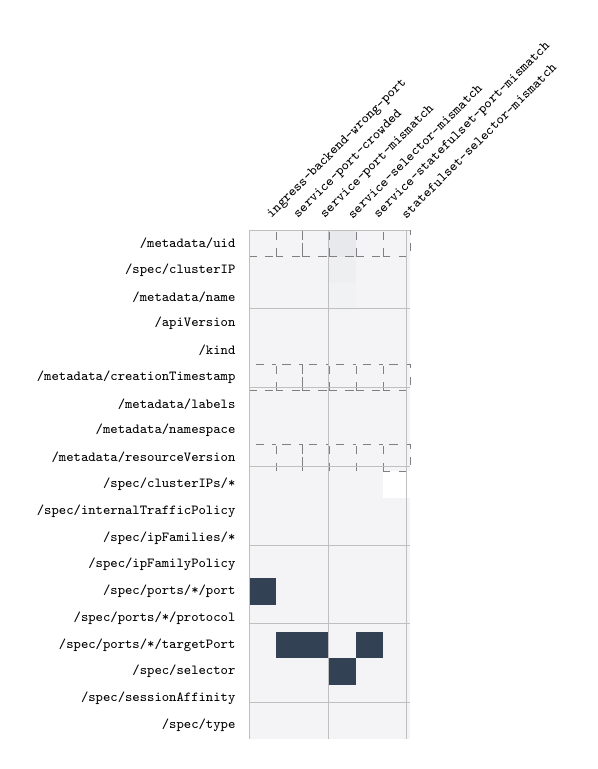
\begin{tikzpicture}[x=3.4mm,y=3.4mm]
\node[rotate=45,anchor=west,font=\ttfamily\tiny] at (0.5,0.25) {ingress-backend-wrong-port};
\node[rotate=45,anchor=west,font=\ttfamily\tiny] at (1.5,0.25) {service-port-crowded};
\node[rotate=45,anchor=west,font=\ttfamily\tiny] at (2.5,0.25) {service-port-mismatch};
\node[rotate=45,anchor=west,font=\ttfamily\tiny] at (3.5,0.25) {service-selector-mismatch};
\node[rotate=45,anchor=west,font=\ttfamily\tiny] at (4.5,0.25) {service-statefulset-port-mismatch};
\node[rotate=45,anchor=west,font=\ttfamily\tiny] at (5.5,0.25) {statefulset-selector-mismatch};
\node[anchor=east,font=\ttfamily\tiny] at (-0.15,-0.5) {/metadata/uid};
\fill[fill={rgb,255:red,244;green,244;blue,246}] (0,-1) rectangle ++(1,1);
\draw[gray,dashed,line width=0.2pt] (0,-1) rectangle ++(1,1);
\fill[fill={rgb,255:red,244;green,244;blue,246}] (1,-1) rectangle ++(1,1);
\draw[gray,dashed,line width=0.2pt] (1,-1) rectangle ++(1,1);
\fill[fill={rgb,255:red,244;green,244;blue,246}] (2,-1) rectangle ++(1,1);
\draw[gray,dashed,line width=0.2pt] (2,-1) rectangle ++(1,1);
\fill[fill={rgb,255:red,232;green,233;blue,236}] (3,-1) rectangle ++(1,1);
\draw[gray,dashed,line width=0.2pt] (3,-1) rectangle ++(1,1);
\fill[fill={rgb,255:red,244;green,244;blue,246}] (4,-1) rectangle ++(1,1);
\draw[gray,dashed,line width=0.2pt] (4,-1) rectangle ++(1,1);
\fill[fill={rgb,255:red,244;green,244;blue,246}] (5,-1) rectangle ++(1,1);
\draw[gray,dashed,line width=0.2pt] (5,-1) rectangle ++(1,1);
\node[anchor=east,font=\ttfamily\tiny] at (-0.15,-1.5) {/spec/clusterIP};
\fill[fill={rgb,255:red,244;green,244;blue,246}] (0,-2) rectangle ++(1,1);
\fill[fill={rgb,255:red,244;green,244;blue,246}] (1,-2) rectangle ++(1,1);
\fill[fill={rgb,255:red,244;green,244;blue,246}] (2,-2) rectangle ++(1,1);
\fill[fill={rgb,255:red,238;green,239;blue,241}] (3,-2) rectangle ++(1,1);
\fill[fill={rgb,255:red,244;green,244;blue,246}] (4,-2) rectangle ++(1,1);
\fill[fill={rgb,255:red,244;green,244;blue,246}] (5,-2) rectangle ++(1,1);
\node[anchor=east,font=\ttfamily\tiny] at (-0.15,-2.5) {/metadata/name};
\fill[fill={rgb,255:red,244;green,244;blue,246}] (0,-3) rectangle ++(1,1);
\fill[fill={rgb,255:red,244;green,244;blue,246}] (1,-3) rectangle ++(1,1);
\fill[fill={rgb,255:red,244;green,244;blue,246}] (2,-3) rectangle ++(1,1);
\fill[fill={rgb,255:red,241;green,242;blue,243}] (3,-3) rectangle ++(1,1);
\fill[fill={rgb,255:red,244;green,244;blue,246}] (4,-3) rectangle ++(1,1);
\fill[fill={rgb,255:red,244;green,244;blue,246}] (5,-3) rectangle ++(1,1);
\node[anchor=east,font=\ttfamily\tiny] at (-0.15,-3.5) {/apiVersion};
\fill[fill={rgb,255:red,244;green,244;blue,246}] (0,-4) rectangle ++(1,1);
\fill[fill={rgb,255:red,244;green,244;blue,246}] (1,-4) rectangle ++(1,1);
\fill[fill={rgb,255:red,244;green,244;blue,246}] (2,-4) rectangle ++(1,1);
\fill[fill={rgb,255:red,244;green,244;blue,246}] (3,-4) rectangle ++(1,1);
\fill[fill={rgb,255:red,244;green,244;blue,246}] (4,-4) rectangle ++(1,1);
\fill[fill={rgb,255:red,244;green,244;blue,246}] (5,-4) rectangle ++(1,1);
\node[anchor=east,font=\ttfamily\tiny] at (-0.15,-4.5) {/kind};
\fill[fill={rgb,255:red,244;green,244;blue,246}] (0,-5) rectangle ++(1,1);
\fill[fill={rgb,255:red,244;green,244;blue,246}] (1,-5) rectangle ++(1,1);
\fill[fill={rgb,255:red,244;green,244;blue,246}] (2,-5) rectangle ++(1,1);
\fill[fill={rgb,255:red,244;green,244;blue,246}] (3,-5) rectangle ++(1,1);
\fill[fill={rgb,255:red,244;green,244;blue,246}] (4,-5) rectangle ++(1,1);
\fill[fill={rgb,255:red,244;green,244;blue,246}] (5,-5) rectangle ++(1,1);
\node[anchor=east,font=\ttfamily\tiny] at (-0.15,-5.5) {/metadata/creationTimestamp};
\fill[fill={rgb,255:red,244;green,244;blue,246}] (0,-6) rectangle ++(1,1);
\draw[gray,dashed,line width=0.2pt] (0,-6) rectangle ++(1,1);
\fill[fill={rgb,255:red,244;green,244;blue,246}] (1,-6) rectangle ++(1,1);
\draw[gray,dashed,line width=0.2pt] (1,-6) rectangle ++(1,1);
\fill[fill={rgb,255:red,244;green,244;blue,246}] (2,-6) rectangle ++(1,1);
\draw[gray,dashed,line width=0.2pt] (2,-6) rectangle ++(1,1);
\fill[fill={rgb,255:red,244;green,244;blue,246}] (3,-6) rectangle ++(1,1);
\draw[gray,dashed,line width=0.2pt] (3,-6) rectangle ++(1,1);
\fill[fill={rgb,255:red,244;green,244;blue,246}] (4,-6) rectangle ++(1,1);
\draw[gray,dashed,line width=0.2pt] (4,-6) rectangle ++(1,1);
\fill[fill={rgb,255:red,244;green,244;blue,246}] (5,-6) rectangle ++(1,1);
\draw[gray,dashed,line width=0.2pt] (5,-6) rectangle ++(1,1);
\node[anchor=east,font=\ttfamily\tiny] at (-0.15,-6.5) {/metadata/labels};
\fill[fill={rgb,255:red,244;green,244;blue,246}] (0,-7) rectangle ++(1,1);
\fill[fill={rgb,255:red,244;green,244;blue,246}] (1,-7) rectangle ++(1,1);
\fill[fill={rgb,255:red,244;green,244;blue,246}] (2,-7) rectangle ++(1,1);
\fill[fill={rgb,255:red,244;green,244;blue,246}] (3,-7) rectangle ++(1,1);
\fill[fill={rgb,255:red,244;green,244;blue,246}] (4,-7) rectangle ++(1,1);
\fill[fill={rgb,255:red,244;green,244;blue,246}] (5,-7) rectangle ++(1,1);
\node[anchor=east,font=\ttfamily\tiny] at (-0.15,-7.5) {/metadata/namespace};
\fill[fill={rgb,255:red,244;green,244;blue,246}] (0,-8) rectangle ++(1,1);
\fill[fill={rgb,255:red,244;green,244;blue,246}] (1,-8) rectangle ++(1,1);
\fill[fill={rgb,255:red,244;green,244;blue,246}] (2,-8) rectangle ++(1,1);
\fill[fill={rgb,255:red,244;green,244;blue,246}] (3,-8) rectangle ++(1,1);
\fill[fill={rgb,255:red,244;green,244;blue,246}] (4,-8) rectangle ++(1,1);
\fill[fill={rgb,255:red,244;green,244;blue,246}] (5,-8) rectangle ++(1,1);
\node[anchor=east,font=\ttfamily\tiny] at (-0.15,-8.5) {/metadata/resourceVersion};
\fill[fill={rgb,255:red,244;green,244;blue,246}] (0,-9) rectangle ++(1,1);
\draw[gray,dashed,line width=0.2pt] (0,-9) rectangle ++(1,1);
\fill[fill={rgb,255:red,244;green,244;blue,246}] (1,-9) rectangle ++(1,1);
\draw[gray,dashed,line width=0.2pt] (1,-9) rectangle ++(1,1);
\fill[fill={rgb,255:red,244;green,244;blue,246}] (2,-9) rectangle ++(1,1);
\draw[gray,dashed,line width=0.2pt] (2,-9) rectangle ++(1,1);
\fill[fill={rgb,255:red,244;green,244;blue,246}] (3,-9) rectangle ++(1,1);
\draw[gray,dashed,line width=0.2pt] (3,-9) rectangle ++(1,1);
\fill[fill={rgb,255:red,244;green,244;blue,246}] (4,-9) rectangle ++(1,1);
\draw[gray,dashed,line width=0.2pt] (4,-9) rectangle ++(1,1);
\fill[fill={rgb,255:red,244;green,244;blue,246}] (5,-9) rectangle ++(1,1);
\draw[gray,dashed,line width=0.2pt] (5,-9) rectangle ++(1,1);
\node[anchor=east,font=\ttfamily\tiny] at (-0.15,-9.5) {/spec/clusterIPs/*};
\fill[fill={rgb,255:red,244;green,244;blue,246}] (0,-10) rectangle ++(1,1);
\fill[fill={rgb,255:red,244;green,244;blue,246}] (1,-10) rectangle ++(1,1);
\fill[fill={rgb,255:red,244;green,244;blue,246}] (2,-10) rectangle ++(1,1);
\fill[fill={rgb,255:red,244;green,244;blue,246}] (3,-10) rectangle ++(1,1);
\fill[fill={rgb,255:red,244;green,244;blue,246}] (4,-10) rectangle ++(1,1);
\node[anchor=east,font=\ttfamily\tiny] at (-0.15,-10.5) {/spec/internalTrafficPolicy};
\fill[fill={rgb,255:red,244;green,244;blue,246}] (0,-11) rectangle ++(1,1);
\fill[fill={rgb,255:red,244;green,244;blue,246}] (1,-11) rectangle ++(1,1);
\fill[fill={rgb,255:red,244;green,244;blue,246}] (2,-11) rectangle ++(1,1);
\fill[fill={rgb,255:red,244;green,244;blue,246}] (3,-11) rectangle ++(1,1);
\fill[fill={rgb,255:red,244;green,244;blue,246}] (4,-11) rectangle ++(1,1);
\fill[fill={rgb,255:red,244;green,244;blue,246}] (5,-11) rectangle ++(1,1);
\node[anchor=east,font=\ttfamily\tiny] at (-0.15,-11.5) {/spec/ipFamilies/*};
\fill[fill={rgb,255:red,244;green,244;blue,246}] (0,-12) rectangle ++(1,1);
\fill[fill={rgb,255:red,244;green,244;blue,246}] (1,-12) rectangle ++(1,1);
\fill[fill={rgb,255:red,244;green,244;blue,246}] (2,-12) rectangle ++(1,1);
\fill[fill={rgb,255:red,244;green,244;blue,246}] (3,-12) rectangle ++(1,1);
\fill[fill={rgb,255:red,244;green,244;blue,246}] (4,-12) rectangle ++(1,1);
\fill[fill={rgb,255:red,244;green,244;blue,246}] (5,-12) rectangle ++(1,1);
\node[anchor=east,font=\ttfamily\tiny] at (-0.15,-12.5) {/spec/ipFamilyPolicy};
\fill[fill={rgb,255:red,244;green,244;blue,246}] (0,-13) rectangle ++(1,1);
\fill[fill={rgb,255:red,244;green,244;blue,246}] (1,-13) rectangle ++(1,1);
\fill[fill={rgb,255:red,244;green,244;blue,246}] (2,-13) rectangle ++(1,1);
\fill[fill={rgb,255:red,244;green,244;blue,246}] (3,-13) rectangle ++(1,1);
\fill[fill={rgb,255:red,244;green,244;blue,246}] (4,-13) rectangle ++(1,1);
\fill[fill={rgb,255:red,244;green,244;blue,246}] (5,-13) rectangle ++(1,1);
\node[anchor=east,font=\ttfamily\tiny] at (-0.15,-13.5) {/spec/ports/*/port};
\fill[fill={rgb,255:red,51;green,65;blue,85}] (0,-14) rectangle ++(1,1);
\node[white,font=\tiny] at (0.5,-14.5) {$\ast$};
\fill[fill={rgb,255:red,244;green,244;blue,246}] (1,-14) rectangle ++(1,1);
\fill[fill={rgb,255:red,244;green,244;blue,246}] (2,-14) rectangle ++(1,1);
\fill[fill={rgb,255:red,244;green,244;blue,246}] (3,-14) rectangle ++(1,1);
\fill[fill={rgb,255:red,244;green,244;blue,246}] (4,-14) rectangle ++(1,1);
\fill[fill={rgb,255:red,244;green,244;blue,246}] (5,-14) rectangle ++(1,1);
\node[anchor=east,font=\ttfamily\tiny] at (-0.15,-14.5) {/spec/ports/*/protocol};
\fill[fill={rgb,255:red,244;green,244;blue,246}] (0,-15) rectangle ++(1,1);
\fill[fill={rgb,255:red,244;green,244;blue,246}] (1,-15) rectangle ++(1,1);
\fill[fill={rgb,255:red,244;green,244;blue,246}] (2,-15) rectangle ++(1,1);
\fill[fill={rgb,255:red,244;green,244;blue,246}] (3,-15) rectangle ++(1,1);
\fill[fill={rgb,255:red,244;green,244;blue,246}] (4,-15) rectangle ++(1,1);
\fill[fill={rgb,255:red,244;green,244;blue,246}] (5,-15) rectangle ++(1,1);
\node[anchor=east,font=\ttfamily\tiny] at (-0.15,-15.5) {/spec/ports/*/targetPort};
\fill[fill={rgb,255:red,244;green,244;blue,246}] (0,-16) rectangle ++(1,1);
\fill[fill={rgb,255:red,51;green,65;blue,85}] (1,-16) rectangle ++(1,1);
\node[white,font=\tiny] at (1.5,-16.5) {$\ast$};
\fill[fill={rgb,255:red,51;green,65;blue,85}] (2,-16) rectangle ++(1,1);
\node[white,font=\tiny] at (2.5,-16.5) {$\ast$};
\fill[fill={rgb,255:red,244;green,244;blue,246}] (3,-16) rectangle ++(1,1);
\fill[fill={rgb,255:red,51;green,65;blue,85}] (4,-16) rectangle ++(1,1);
\node[white,font=\tiny] at (4.5,-16.5) {$\ast$};
\fill[fill={rgb,255:red,244;green,244;blue,246}] (5,-16) rectangle ++(1,1);
\node[anchor=east,font=\ttfamily\tiny] at (-0.15,-16.5) {/spec/selector};
\fill[fill={rgb,255:red,244;green,244;blue,246}] (0,-17) rectangle ++(1,1);
\fill[fill={rgb,255:red,244;green,244;blue,246}] (1,-17) rectangle ++(1,1);
\fill[fill={rgb,255:red,244;green,244;blue,246}] (2,-17) rectangle ++(1,1);
\fill[fill={rgb,255:red,51;green,65;blue,85}] (3,-17) rectangle ++(1,1);
\node[white,font=\tiny] at (3.5,-17.5) {$\ast$};
\fill[fill={rgb,255:red,244;green,244;blue,246}] (4,-17) rectangle ++(1,1);
\fill[fill={rgb,255:red,244;green,244;blue,246}] (5,-17) rectangle ++(1,1);
\node[anchor=east,font=\ttfamily\tiny] at (-0.15,-17.5) {/spec/sessionAffinity};
\fill[fill={rgb,255:red,244;green,244;blue,246}] (0,-18) rectangle ++(1,1);
\fill[fill={rgb,255:red,244;green,244;blue,246}] (1,-18) rectangle ++(1,1);
\fill[fill={rgb,255:red,244;green,244;blue,246}] (2,-18) rectangle ++(1,1);
\fill[fill={rgb,255:red,244;green,244;blue,246}] (3,-18) rectangle ++(1,1);
\fill[fill={rgb,255:red,244;green,244;blue,246}] (4,-18) rectangle ++(1,1);
\fill[fill={rgb,255:red,244;green,244;blue,246}] (5,-18) rectangle ++(1,1);
\node[anchor=east,font=\ttfamily\tiny] at (-0.15,-18.5) {/spec/type};
\fill[fill={rgb,255:red,244;green,244;blue,246}] (0,-19) rectangle ++(1,1);
\fill[fill={rgb,255:red,244;green,244;blue,246}] (1,-19) rectangle ++(1,1);
\fill[fill={rgb,255:red,244;green,244;blue,246}] (2,-19) rectangle ++(1,1);
\fill[fill={rgb,255:red,244;green,244;blue,246}] (3,-19) rectangle ++(1,1);
\fill[fill={rgb,255:red,244;green,244;blue,246}] (4,-19) rectangle ++(1,1);
\fill[fill={rgb,255:red,244;green,244;blue,246}] (5,-19) rectangle ++(1,1);
\draw[gray!50,line width=0.2pt] (0,0) grid (6,-19);
\end{tikzpicture}

\par\medskip\noindent{\small\bfseries ClusterRoleBinding}\par\smallskip
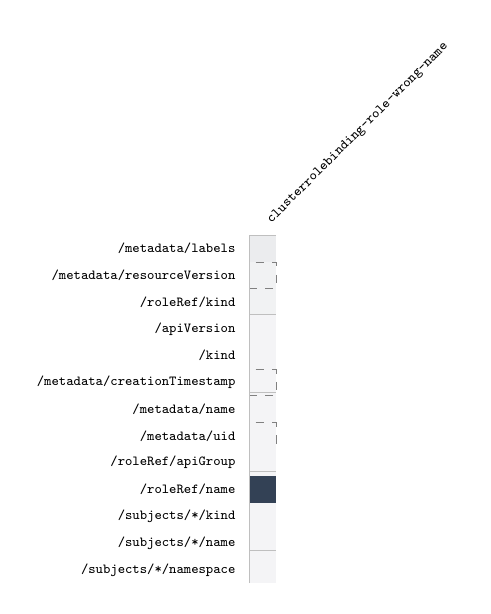
\begin{tikzpicture}[x=3.4mm,y=3.4mm]
\node[rotate=45,anchor=west,font=\ttfamily\tiny] at (0.5,0.25) {clusterrolebinding-role-wrong-name};
\node[anchor=east,font=\ttfamily\tiny] at (-0.15,-0.5) {/metadata/labels};
\fill[fill={rgb,255:red,235;green,236;blue,238}] (0,-1) rectangle ++(1,1);
\node[anchor=east,font=\ttfamily\tiny] at (-0.15,-1.5) {/metadata/resourceVersion};
\fill[fill={rgb,255:red,241;green,242;blue,243}] (0,-2) rectangle ++(1,1);
\draw[gray,dashed,line width=0.2pt] (0,-2) rectangle ++(1,1);
\node[anchor=east,font=\ttfamily\tiny] at (-0.15,-2.5) {/roleRef/kind};
\fill[fill={rgb,255:red,241;green,242;blue,243}] (0,-3) rectangle ++(1,1);
\node[anchor=east,font=\ttfamily\tiny] at (-0.15,-3.5) {/apiVersion};
\fill[fill={rgb,255:red,244;green,244;blue,246}] (0,-4) rectangle ++(1,1);
\node[anchor=east,font=\ttfamily\tiny] at (-0.15,-4.5) {/kind};
\fill[fill={rgb,255:red,244;green,244;blue,246}] (0,-5) rectangle ++(1,1);
\node[anchor=east,font=\ttfamily\tiny] at (-0.15,-5.5) {/metadata/creationTimestamp};
\fill[fill={rgb,255:red,244;green,244;blue,246}] (0,-6) rectangle ++(1,1);
\draw[gray,dashed,line width=0.2pt] (0,-6) rectangle ++(1,1);
\node[anchor=east,font=\ttfamily\tiny] at (-0.15,-6.5) {/metadata/name};
\fill[fill={rgb,255:red,244;green,244;blue,246}] (0,-7) rectangle ++(1,1);
\node[anchor=east,font=\ttfamily\tiny] at (-0.15,-7.5) {/metadata/uid};
\fill[fill={rgb,255:red,244;green,244;blue,246}] (0,-8) rectangle ++(1,1);
\draw[gray,dashed,line width=0.2pt] (0,-8) rectangle ++(1,1);
\node[anchor=east,font=\ttfamily\tiny] at (-0.15,-8.5) {/roleRef/apiGroup};
\fill[fill={rgb,255:red,244;green,244;blue,246}] (0,-9) rectangle ++(1,1);
\node[anchor=east,font=\ttfamily\tiny] at (-0.15,-9.5) {/roleRef/name};
\fill[fill={rgb,255:red,51;green,65;blue,85}] (0,-10) rectangle ++(1,1);
\node[white,font=\tiny] at (0.5,-10.5) {$\ast$};
\node[anchor=east,font=\ttfamily\tiny] at (-0.15,-10.5) {/subjects/*/kind};
\fill[fill={rgb,255:red,244;green,244;blue,246}] (0,-11) rectangle ++(1,1);
\node[anchor=east,font=\ttfamily\tiny] at (-0.15,-11.5) {/subjects/*/name};
\fill[fill={rgb,255:red,244;green,244;blue,246}] (0,-12) rectangle ++(1,1);
\node[anchor=east,font=\ttfamily\tiny] at (-0.15,-12.5) {/subjects/*/namespace};
\fill[fill={rgb,255:red,244;green,244;blue,246}] (0,-13) rectangle ++(1,1);
\draw[gray!50,line width=0.2pt] (0,0) grid (1,-13);
\end{tikzpicture}

\par\medskip\noindent{\small\bfseries ConfigMap}\par\smallskip
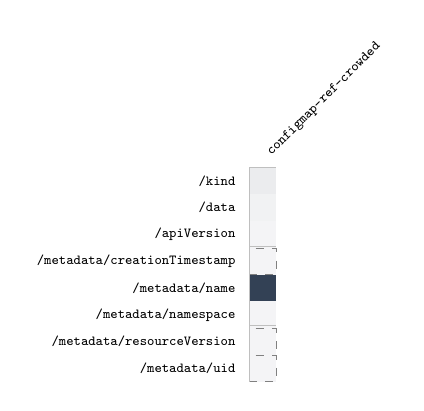
\begin{tikzpicture}[x=3.4mm,y=3.4mm]
\node[rotate=45,anchor=west,font=\ttfamily\tiny] at (0.5,0.25) {configmap-ref-crowded};
\node[anchor=east,font=\ttfamily\tiny] at (-0.15,-0.5) {/kind};
\fill[fill={rgb,255:red,235;green,236;blue,238}] (0,-1) rectangle ++(1,1);
\node[anchor=east,font=\ttfamily\tiny] at (-0.15,-1.5) {/data};
\fill[fill={rgb,255:red,241;green,242;blue,243}] (0,-2) rectangle ++(1,1);
\node[anchor=east,font=\ttfamily\tiny] at (-0.15,-2.5) {/apiVersion};
\fill[fill={rgb,255:red,244;green,244;blue,246}] (0,-3) rectangle ++(1,1);
\node[anchor=east,font=\ttfamily\tiny] at (-0.15,-3.5) {/metadata/creationTimestamp};
\fill[fill={rgb,255:red,244;green,244;blue,246}] (0,-4) rectangle ++(1,1);
\draw[gray,dashed,line width=0.2pt] (0,-4) rectangle ++(1,1);
\node[anchor=east,font=\ttfamily\tiny] at (-0.15,-4.5) {/metadata/name};
\fill[fill={rgb,255:red,51;green,65;blue,85}] (0,-5) rectangle ++(1,1);
\node[white,font=\tiny] at (0.5,-5.5) {$\ast$};
\node[anchor=east,font=\ttfamily\tiny] at (-0.15,-5.5) {/metadata/namespace};
\fill[fill={rgb,255:red,244;green,244;blue,246}] (0,-6) rectangle ++(1,1);
\node[anchor=east,font=\ttfamily\tiny] at (-0.15,-6.5) {/metadata/resourceVersion};
\fill[fill={rgb,255:red,244;green,244;blue,246}] (0,-7) rectangle ++(1,1);
\draw[gray,dashed,line width=0.2pt] (0,-7) rectangle ++(1,1);
\node[anchor=east,font=\ttfamily\tiny] at (-0.15,-7.5) {/metadata/uid};
\fill[fill={rgb,255:red,244;green,244;blue,246}] (0,-8) rectangle ++(1,1);
\draw[gray,dashed,line width=0.2pt] (0,-8) rectangle ++(1,1);
\draw[gray!50,line width=0.2pt] (0,0) grid (1,-8);
\end{tikzpicture}

\par\medskip\noindent{\small\bfseries Deployment}\par\smallskip
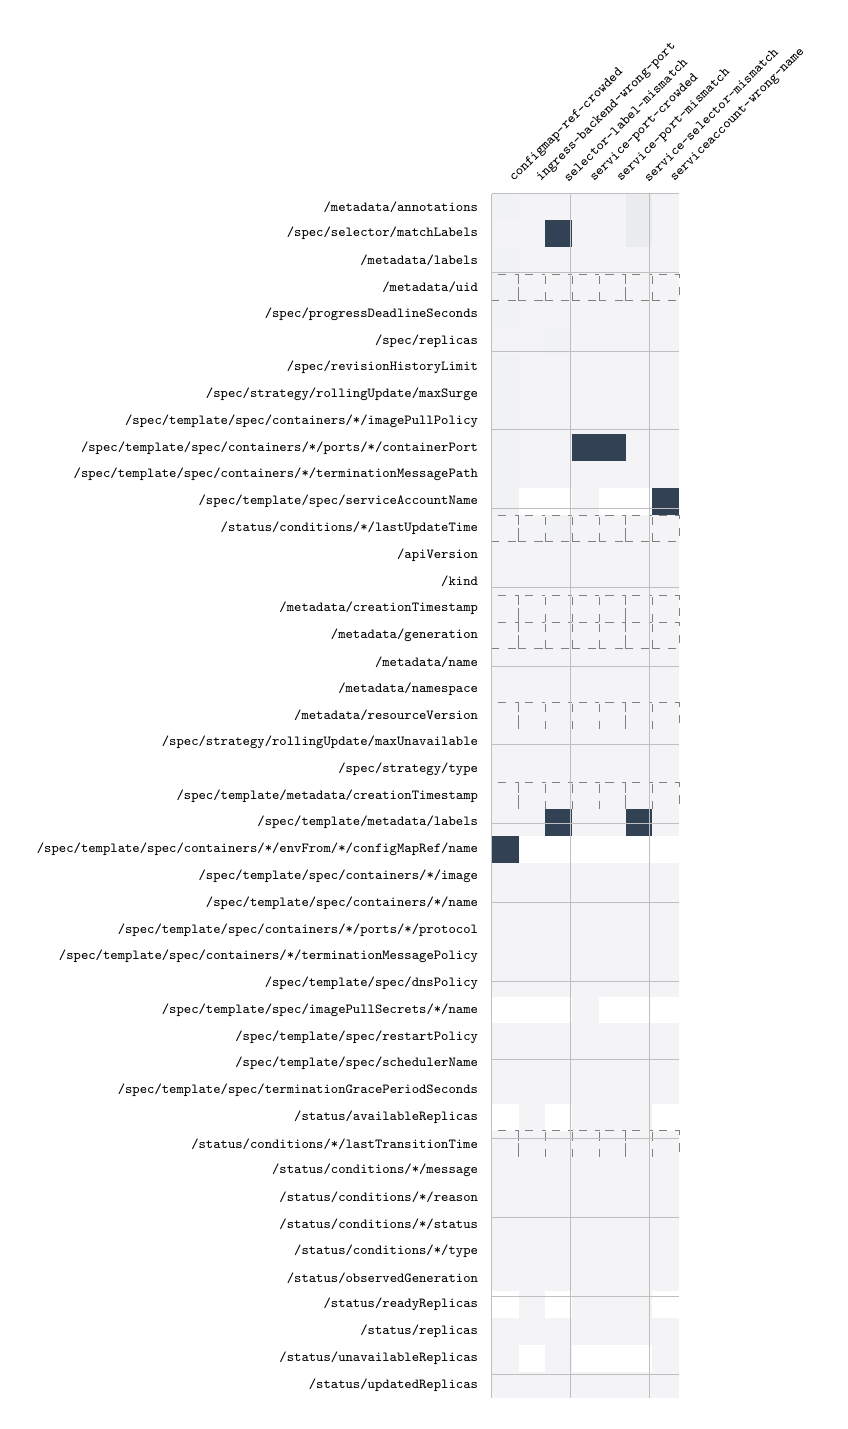
\begin{tikzpicture}[x=3.4mm,y=3.4mm]
\node[rotate=45,anchor=west,font=\ttfamily\tiny] at (0.5,0.25) {configmap-ref-crowded};
\node[rotate=45,anchor=west,font=\ttfamily\tiny] at (1.5,0.25) {ingress-backend-wrong-port};
\node[rotate=45,anchor=west,font=\ttfamily\tiny] at (2.5,0.25) {selector-label-mismatch};
\node[rotate=45,anchor=west,font=\ttfamily\tiny] at (3.5,0.25) {service-port-crowded};
\node[rotate=45,anchor=west,font=\ttfamily\tiny] at (4.5,0.25) {service-port-mismatch};
\node[rotate=45,anchor=west,font=\ttfamily\tiny] at (5.5,0.25) {service-selector-mismatch};
\node[rotate=45,anchor=west,font=\ttfamily\tiny] at (6.5,0.25) {serviceaccount-wrong-name};
\node[anchor=east,font=\ttfamily\tiny] at (-0.15,-0.5) {/metadata/annotations};
\fill[fill={rgb,255:red,241;green,242;blue,243}] (0,-1) rectangle ++(1,1);
\fill[fill={rgb,255:red,244;green,244;blue,246}] (1,-1) rectangle ++(1,1);
\fill[fill={rgb,255:red,244;green,244;blue,246}] (2,-1) rectangle ++(1,1);
\fill[fill={rgb,255:red,244;green,244;blue,246}] (3,-1) rectangle ++(1,1);
\fill[fill={rgb,255:red,244;green,244;blue,246}] (4,-1) rectangle ++(1,1);
\fill[fill={rgb,255:red,235;green,236;blue,238}] (5,-1) rectangle ++(1,1);
\fill[fill={rgb,255:red,244;green,244;blue,246}] (6,-1) rectangle ++(1,1);
\node[anchor=east,font=\ttfamily\tiny] at (-0.15,-1.5) {/spec/selector/matchLabels};
\fill[fill={rgb,255:red,244;green,244;blue,246}] (0,-2) rectangle ++(1,1);
\fill[fill={rgb,255:red,244;green,244;blue,246}] (1,-2) rectangle ++(1,1);
\fill[fill={rgb,255:red,51;green,65;blue,85}] (2,-2) rectangle ++(1,1);
\node[white,font=\tiny] at (2.5,-2.5) {$\ast$};
\fill[fill={rgb,255:red,244;green,244;blue,246}] (3,-2) rectangle ++(1,1);
\fill[fill={rgb,255:red,244;green,244;blue,246}] (4,-2) rectangle ++(1,1);
\fill[fill={rgb,255:red,235;green,236;blue,238}] (5,-2) rectangle ++(1,1);
\fill[fill={rgb,255:red,244;green,244;blue,246}] (6,-2) rectangle ++(1,1);
\node[anchor=east,font=\ttfamily\tiny] at (-0.15,-2.5) {/metadata/labels};
\fill[fill={rgb,255:red,241;green,242;blue,243}] (0,-3) rectangle ++(1,1);
\fill[fill={rgb,255:red,244;green,244;blue,246}] (1,-3) rectangle ++(1,1);
\fill[fill={rgb,255:red,244;green,244;blue,246}] (2,-3) rectangle ++(1,1);
\fill[fill={rgb,255:red,244;green,244;blue,246}] (3,-3) rectangle ++(1,1);
\fill[fill={rgb,255:red,244;green,244;blue,246}] (4,-3) rectangle ++(1,1);
\fill[fill={rgb,255:red,244;green,244;blue,246}] (5,-3) rectangle ++(1,1);
\fill[fill={rgb,255:red,244;green,244;blue,246}] (6,-3) rectangle ++(1,1);
\node[anchor=east,font=\ttfamily\tiny] at (-0.15,-3.5) {/metadata/uid};
\fill[fill={rgb,255:red,241;green,242;blue,243}] (0,-4) rectangle ++(1,1);
\draw[gray,dashed,line width=0.2pt] (0,-4) rectangle ++(1,1);
\fill[fill={rgb,255:red,244;green,244;blue,246}] (1,-4) rectangle ++(1,1);
\draw[gray,dashed,line width=0.2pt] (1,-4) rectangle ++(1,1);
\fill[fill={rgb,255:red,244;green,244;blue,246}] (2,-4) rectangle ++(1,1);
\draw[gray,dashed,line width=0.2pt] (2,-4) rectangle ++(1,1);
\fill[fill={rgb,255:red,244;green,244;blue,246}] (3,-4) rectangle ++(1,1);
\draw[gray,dashed,line width=0.2pt] (3,-4) rectangle ++(1,1);
\fill[fill={rgb,255:red,244;green,244;blue,246}] (4,-4) rectangle ++(1,1);
\draw[gray,dashed,line width=0.2pt] (4,-4) rectangle ++(1,1);
\fill[fill={rgb,255:red,244;green,244;blue,246}] (5,-4) rectangle ++(1,1);
\draw[gray,dashed,line width=0.2pt] (5,-4) rectangle ++(1,1);
\fill[fill={rgb,255:red,244;green,244;blue,246}] (6,-4) rectangle ++(1,1);
\draw[gray,dashed,line width=0.2pt] (6,-4) rectangle ++(1,1);
\node[anchor=east,font=\ttfamily\tiny] at (-0.15,-4.5) {/spec/progressDeadlineSeconds};
\fill[fill={rgb,255:red,241;green,242;blue,243}] (0,-5) rectangle ++(1,1);
\fill[fill={rgb,255:red,244;green,244;blue,246}] (1,-5) rectangle ++(1,1);
\fill[fill={rgb,255:red,244;green,244;blue,246}] (2,-5) rectangle ++(1,1);
\fill[fill={rgb,255:red,244;green,244;blue,246}] (3,-5) rectangle ++(1,1);
\fill[fill={rgb,255:red,244;green,244;blue,246}] (4,-5) rectangle ++(1,1);
\fill[fill={rgb,255:red,244;green,244;blue,246}] (5,-5) rectangle ++(1,1);
\fill[fill={rgb,255:red,244;green,244;blue,246}] (6,-5) rectangle ++(1,1);
\node[anchor=east,font=\ttfamily\tiny] at (-0.15,-5.5) {/spec/replicas};
\fill[fill={rgb,255:red,244;green,244;blue,246}] (0,-6) rectangle ++(1,1);
\fill[fill={rgb,255:red,244;green,244;blue,246}] (1,-6) rectangle ++(1,1);
\fill[fill={rgb,255:red,241;green,242;blue,243}] (2,-6) rectangle ++(1,1);
\fill[fill={rgb,255:red,244;green,244;blue,246}] (3,-6) rectangle ++(1,1);
\fill[fill={rgb,255:red,244;green,244;blue,246}] (4,-6) rectangle ++(1,1);
\fill[fill={rgb,255:red,244;green,244;blue,246}] (5,-6) rectangle ++(1,1);
\fill[fill={rgb,255:red,244;green,244;blue,246}] (6,-6) rectangle ++(1,1);
\node[anchor=east,font=\ttfamily\tiny] at (-0.15,-6.5) {/spec/revisionHistoryLimit};
\fill[fill={rgb,255:red,241;green,242;blue,243}] (0,-7) rectangle ++(1,1);
\fill[fill={rgb,255:red,244;green,244;blue,246}] (1,-7) rectangle ++(1,1);
\fill[fill={rgb,255:red,244;green,244;blue,246}] (2,-7) rectangle ++(1,1);
\fill[fill={rgb,255:red,244;green,244;blue,246}] (3,-7) rectangle ++(1,1);
\fill[fill={rgb,255:red,244;green,244;blue,246}] (4,-7) rectangle ++(1,1);
\fill[fill={rgb,255:red,244;green,244;blue,246}] (5,-7) rectangle ++(1,1);
\fill[fill={rgb,255:red,244;green,244;blue,246}] (6,-7) rectangle ++(1,1);
\node[anchor=east,font=\ttfamily\tiny] at (-0.15,-7.5) {/spec/strategy/rollingUpdate/maxSurge};
\fill[fill={rgb,255:red,241;green,242;blue,243}] (0,-8) rectangle ++(1,1);
\fill[fill={rgb,255:red,244;green,244;blue,246}] (1,-8) rectangle ++(1,1);
\fill[fill={rgb,255:red,244;green,244;blue,246}] (2,-8) rectangle ++(1,1);
\fill[fill={rgb,255:red,244;green,244;blue,246}] (3,-8) rectangle ++(1,1);
\fill[fill={rgb,255:red,244;green,244;blue,246}] (4,-8) rectangle ++(1,1);
\fill[fill={rgb,255:red,244;green,244;blue,246}] (5,-8) rectangle ++(1,1);
\fill[fill={rgb,255:red,244;green,244;blue,246}] (6,-8) rectangle ++(1,1);
\node[anchor=east,font=\ttfamily\tiny] at (-0.15,-8.5) {/spec/template/spec/containers/*/imagePullPolicy};
\fill[fill={rgb,255:red,241;green,242;blue,243}] (0,-9) rectangle ++(1,1);
\fill[fill={rgb,255:red,244;green,244;blue,246}] (1,-9) rectangle ++(1,1);
\fill[fill={rgb,255:red,244;green,244;blue,246}] (2,-9) rectangle ++(1,1);
\fill[fill={rgb,255:red,244;green,244;blue,246}] (3,-9) rectangle ++(1,1);
\fill[fill={rgb,255:red,244;green,244;blue,246}] (4,-9) rectangle ++(1,1);
\fill[fill={rgb,255:red,244;green,244;blue,246}] (5,-9) rectangle ++(1,1);
\fill[fill={rgb,255:red,244;green,244;blue,246}] (6,-9) rectangle ++(1,1);
\node[anchor=east,font=\ttfamily\tiny] at (-0.15,-9.5) {/spec/template/spec/containers/*/ports/*/containerPort};
\fill[fill={rgb,255:red,241;green,242;blue,243}] (0,-10) rectangle ++(1,1);
\fill[fill={rgb,255:red,244;green,244;blue,246}] (1,-10) rectangle ++(1,1);
\fill[fill={rgb,255:red,244;green,244;blue,246}] (2,-10) rectangle ++(1,1);
\fill[fill={rgb,255:red,51;green,65;blue,85}] (3,-10) rectangle ++(1,1);
\node[white,font=\tiny] at (3.5,-10.5) {$\ast$};
\fill[fill={rgb,255:red,51;green,65;blue,85}] (4,-10) rectangle ++(1,1);
\node[white,font=\tiny] at (4.5,-10.5) {$\ast$};
\fill[fill={rgb,255:red,244;green,244;blue,246}] (5,-10) rectangle ++(1,1);
\fill[fill={rgb,255:red,244;green,244;blue,246}] (6,-10) rectangle ++(1,1);
\node[anchor=east,font=\ttfamily\tiny] at (-0.15,-10.5) {/spec/template/spec/containers/*/terminationMessagePath};
\fill[fill={rgb,255:red,241;green,242;blue,243}] (0,-11) rectangle ++(1,1);
\fill[fill={rgb,255:red,244;green,244;blue,246}] (1,-11) rectangle ++(1,1);
\fill[fill={rgb,255:red,244;green,244;blue,246}] (2,-11) rectangle ++(1,1);
\fill[fill={rgb,255:red,244;green,244;blue,246}] (3,-11) rectangle ++(1,1);
\fill[fill={rgb,255:red,244;green,244;blue,246}] (4,-11) rectangle ++(1,1);
\fill[fill={rgb,255:red,244;green,244;blue,246}] (5,-11) rectangle ++(1,1);
\fill[fill={rgb,255:red,244;green,244;blue,246}] (6,-11) rectangle ++(1,1);
\node[anchor=east,font=\ttfamily\tiny] at (-0.15,-11.5) {/spec/template/spec/serviceAccountName};
\fill[fill={rgb,255:red,241;green,242;blue,243}] (0,-12) rectangle ++(1,1);
\fill[fill={rgb,255:red,244;green,244;blue,246}] (3,-12) rectangle ++(1,1);
\fill[fill={rgb,255:red,51;green,65;blue,85}] (6,-12) rectangle ++(1,1);
\node[white,font=\tiny] at (6.5,-12.5) {$\ast$};
\node[anchor=east,font=\ttfamily\tiny] at (-0.15,-12.5) {/status/conditions/*/lastUpdateTime};
\fill[fill={rgb,255:red,244;green,244;blue,246}] (0,-13) rectangle ++(1,1);
\draw[gray,dashed,line width=0.2pt] (0,-13) rectangle ++(1,1);
\fill[fill={rgb,255:red,244;green,244;blue,246}] (1,-13) rectangle ++(1,1);
\draw[gray,dashed,line width=0.2pt] (1,-13) rectangle ++(1,1);
\fill[fill={rgb,255:red,241;green,242;blue,243}] (2,-13) rectangle ++(1,1);
\draw[gray,dashed,line width=0.2pt] (2,-13) rectangle ++(1,1);
\fill[fill={rgb,255:red,244;green,244;blue,246}] (3,-13) rectangle ++(1,1);
\draw[gray,dashed,line width=0.2pt] (3,-13) rectangle ++(1,1);
\fill[fill={rgb,255:red,244;green,244;blue,246}] (4,-13) rectangle ++(1,1);
\draw[gray,dashed,line width=0.2pt] (4,-13) rectangle ++(1,1);
\fill[fill={rgb,255:red,244;green,244;blue,246}] (5,-13) rectangle ++(1,1);
\draw[gray,dashed,line width=0.2pt] (5,-13) rectangle ++(1,1);
\fill[fill={rgb,255:red,244;green,244;blue,246}] (6,-13) rectangle ++(1,1);
\draw[gray,dashed,line width=0.2pt] (6,-13) rectangle ++(1,1);
\node[anchor=east,font=\ttfamily\tiny] at (-0.15,-13.5) {/apiVersion};
\fill[fill={rgb,255:red,244;green,244;blue,246}] (0,-14) rectangle ++(1,1);
\fill[fill={rgb,255:red,244;green,244;blue,246}] (1,-14) rectangle ++(1,1);
\fill[fill={rgb,255:red,244;green,244;blue,246}] (2,-14) rectangle ++(1,1);
\fill[fill={rgb,255:red,244;green,244;blue,246}] (3,-14) rectangle ++(1,1);
\fill[fill={rgb,255:red,244;green,244;blue,246}] (4,-14) rectangle ++(1,1);
\fill[fill={rgb,255:red,244;green,244;blue,246}] (5,-14) rectangle ++(1,1);
\fill[fill={rgb,255:red,244;green,244;blue,246}] (6,-14) rectangle ++(1,1);
\node[anchor=east,font=\ttfamily\tiny] at (-0.15,-14.5) {/kind};
\fill[fill={rgb,255:red,244;green,244;blue,246}] (0,-15) rectangle ++(1,1);
\fill[fill={rgb,255:red,244;green,244;blue,246}] (1,-15) rectangle ++(1,1);
\fill[fill={rgb,255:red,244;green,244;blue,246}] (2,-15) rectangle ++(1,1);
\fill[fill={rgb,255:red,244;green,244;blue,246}] (3,-15) rectangle ++(1,1);
\fill[fill={rgb,255:red,244;green,244;blue,246}] (4,-15) rectangle ++(1,1);
\fill[fill={rgb,255:red,244;green,244;blue,246}] (5,-15) rectangle ++(1,1);
\fill[fill={rgb,255:red,244;green,244;blue,246}] (6,-15) rectangle ++(1,1);
\node[anchor=east,font=\ttfamily\tiny] at (-0.15,-15.5) {/metadata/creationTimestamp};
\fill[fill={rgb,255:red,244;green,244;blue,246}] (0,-16) rectangle ++(1,1);
\draw[gray,dashed,line width=0.2pt] (0,-16) rectangle ++(1,1);
\fill[fill={rgb,255:red,244;green,244;blue,246}] (1,-16) rectangle ++(1,1);
\draw[gray,dashed,line width=0.2pt] (1,-16) rectangle ++(1,1);
\fill[fill={rgb,255:red,244;green,244;blue,246}] (2,-16) rectangle ++(1,1);
\draw[gray,dashed,line width=0.2pt] (2,-16) rectangle ++(1,1);
\fill[fill={rgb,255:red,244;green,244;blue,246}] (3,-16) rectangle ++(1,1);
\draw[gray,dashed,line width=0.2pt] (3,-16) rectangle ++(1,1);
\fill[fill={rgb,255:red,244;green,244;blue,246}] (4,-16) rectangle ++(1,1);
\draw[gray,dashed,line width=0.2pt] (4,-16) rectangle ++(1,1);
\fill[fill={rgb,255:red,244;green,244;blue,246}] (5,-16) rectangle ++(1,1);
\draw[gray,dashed,line width=0.2pt] (5,-16) rectangle ++(1,1);
\fill[fill={rgb,255:red,244;green,244;blue,246}] (6,-16) rectangle ++(1,1);
\draw[gray,dashed,line width=0.2pt] (6,-16) rectangle ++(1,1);
\node[anchor=east,font=\ttfamily\tiny] at (-0.15,-16.5) {/metadata/generation};
\fill[fill={rgb,255:red,244;green,244;blue,246}] (0,-17) rectangle ++(1,1);
\draw[gray,dashed,line width=0.2pt] (0,-17) rectangle ++(1,1);
\fill[fill={rgb,255:red,244;green,244;blue,246}] (1,-17) rectangle ++(1,1);
\draw[gray,dashed,line width=0.2pt] (1,-17) rectangle ++(1,1);
\fill[fill={rgb,255:red,244;green,244;blue,246}] (2,-17) rectangle ++(1,1);
\draw[gray,dashed,line width=0.2pt] (2,-17) rectangle ++(1,1);
\fill[fill={rgb,255:red,244;green,244;blue,246}] (3,-17) rectangle ++(1,1);
\draw[gray,dashed,line width=0.2pt] (3,-17) rectangle ++(1,1);
\fill[fill={rgb,255:red,244;green,244;blue,246}] (4,-17) rectangle ++(1,1);
\draw[gray,dashed,line width=0.2pt] (4,-17) rectangle ++(1,1);
\fill[fill={rgb,255:red,244;green,244;blue,246}] (5,-17) rectangle ++(1,1);
\draw[gray,dashed,line width=0.2pt] (5,-17) rectangle ++(1,1);
\fill[fill={rgb,255:red,244;green,244;blue,246}] (6,-17) rectangle ++(1,1);
\draw[gray,dashed,line width=0.2pt] (6,-17) rectangle ++(1,1);
\node[anchor=east,font=\ttfamily\tiny] at (-0.15,-17.5) {/metadata/name};
\fill[fill={rgb,255:red,244;green,244;blue,246}] (0,-18) rectangle ++(1,1);
\fill[fill={rgb,255:red,244;green,244;blue,246}] (1,-18) rectangle ++(1,1);
\fill[fill={rgb,255:red,244;green,244;blue,246}] (2,-18) rectangle ++(1,1);
\fill[fill={rgb,255:red,244;green,244;blue,246}] (3,-18) rectangle ++(1,1);
\fill[fill={rgb,255:red,244;green,244;blue,246}] (4,-18) rectangle ++(1,1);
\fill[fill={rgb,255:red,244;green,244;blue,246}] (5,-18) rectangle ++(1,1);
\fill[fill={rgb,255:red,244;green,244;blue,246}] (6,-18) rectangle ++(1,1);
\node[anchor=east,font=\ttfamily\tiny] at (-0.15,-18.5) {/metadata/namespace};
\fill[fill={rgb,255:red,244;green,244;blue,246}] (0,-19) rectangle ++(1,1);
\fill[fill={rgb,255:red,244;green,244;blue,246}] (1,-19) rectangle ++(1,1);
\fill[fill={rgb,255:red,244;green,244;blue,246}] (2,-19) rectangle ++(1,1);
\fill[fill={rgb,255:red,244;green,244;blue,246}] (3,-19) rectangle ++(1,1);
\fill[fill={rgb,255:red,244;green,244;blue,246}] (4,-19) rectangle ++(1,1);
\fill[fill={rgb,255:red,244;green,244;blue,246}] (5,-19) rectangle ++(1,1);
\fill[fill={rgb,255:red,244;green,244;blue,246}] (6,-19) rectangle ++(1,1);
\node[anchor=east,font=\ttfamily\tiny] at (-0.15,-19.5) {/metadata/resourceVersion};
\fill[fill={rgb,255:red,244;green,244;blue,246}] (0,-20) rectangle ++(1,1);
\draw[gray,dashed,line width=0.2pt] (0,-20) rectangle ++(1,1);
\fill[fill={rgb,255:red,244;green,244;blue,246}] (1,-20) rectangle ++(1,1);
\draw[gray,dashed,line width=0.2pt] (1,-20) rectangle ++(1,1);
\fill[fill={rgb,255:red,244;green,244;blue,246}] (2,-20) rectangle ++(1,1);
\draw[gray,dashed,line width=0.2pt] (2,-20) rectangle ++(1,1);
\fill[fill={rgb,255:red,244;green,244;blue,246}] (3,-20) rectangle ++(1,1);
\draw[gray,dashed,line width=0.2pt] (3,-20) rectangle ++(1,1);
\fill[fill={rgb,255:red,244;green,244;blue,246}] (4,-20) rectangle ++(1,1);
\draw[gray,dashed,line width=0.2pt] (4,-20) rectangle ++(1,1);
\fill[fill={rgb,255:red,244;green,244;blue,246}] (5,-20) rectangle ++(1,1);
\draw[gray,dashed,line width=0.2pt] (5,-20) rectangle ++(1,1);
\fill[fill={rgb,255:red,244;green,244;blue,246}] (6,-20) rectangle ++(1,1);
\draw[gray,dashed,line width=0.2pt] (6,-20) rectangle ++(1,1);
\node[anchor=east,font=\ttfamily\tiny] at (-0.15,-20.5) {/spec/strategy/rollingUpdate/maxUnavailable};
\fill[fill={rgb,255:red,244;green,244;blue,246}] (0,-21) rectangle ++(1,1);
\fill[fill={rgb,255:red,244;green,244;blue,246}] (1,-21) rectangle ++(1,1);
\fill[fill={rgb,255:red,244;green,244;blue,246}] (2,-21) rectangle ++(1,1);
\fill[fill={rgb,255:red,244;green,244;blue,246}] (3,-21) rectangle ++(1,1);
\fill[fill={rgb,255:red,244;green,244;blue,246}] (4,-21) rectangle ++(1,1);
\fill[fill={rgb,255:red,244;green,244;blue,246}] (5,-21) rectangle ++(1,1);
\fill[fill={rgb,255:red,244;green,244;blue,246}] (6,-21) rectangle ++(1,1);
\node[anchor=east,font=\ttfamily\tiny] at (-0.15,-21.5) {/spec/strategy/type};
\fill[fill={rgb,255:red,244;green,244;blue,246}] (0,-22) rectangle ++(1,1);
\fill[fill={rgb,255:red,244;green,244;blue,246}] (1,-22) rectangle ++(1,1);
\fill[fill={rgb,255:red,244;green,244;blue,246}] (2,-22) rectangle ++(1,1);
\fill[fill={rgb,255:red,244;green,244;blue,246}] (3,-22) rectangle ++(1,1);
\fill[fill={rgb,255:red,244;green,244;blue,246}] (4,-22) rectangle ++(1,1);
\fill[fill={rgb,255:red,244;green,244;blue,246}] (5,-22) rectangle ++(1,1);
\fill[fill={rgb,255:red,244;green,244;blue,246}] (6,-22) rectangle ++(1,1);
\node[anchor=east,font=\ttfamily\tiny] at (-0.15,-22.5) {/spec/template/metadata/creationTimestamp};
\fill[fill={rgb,255:red,244;green,244;blue,246}] (0,-23) rectangle ++(1,1);
\draw[gray,dashed,line width=0.2pt] (0,-23) rectangle ++(1,1);
\fill[fill={rgb,255:red,244;green,244;blue,246}] (1,-23) rectangle ++(1,1);
\draw[gray,dashed,line width=0.2pt] (1,-23) rectangle ++(1,1);
\fill[fill={rgb,255:red,244;green,244;blue,246}] (2,-23) rectangle ++(1,1);
\draw[gray,dashed,line width=0.2pt] (2,-23) rectangle ++(1,1);
\fill[fill={rgb,255:red,244;green,244;blue,246}] (3,-23) rectangle ++(1,1);
\draw[gray,dashed,line width=0.2pt] (3,-23) rectangle ++(1,1);
\fill[fill={rgb,255:red,244;green,244;blue,246}] (4,-23) rectangle ++(1,1);
\draw[gray,dashed,line width=0.2pt] (4,-23) rectangle ++(1,1);
\fill[fill={rgb,255:red,244;green,244;blue,246}] (5,-23) rectangle ++(1,1);
\draw[gray,dashed,line width=0.2pt] (5,-23) rectangle ++(1,1);
\fill[fill={rgb,255:red,244;green,244;blue,246}] (6,-23) rectangle ++(1,1);
\draw[gray,dashed,line width=0.2pt] (6,-23) rectangle ++(1,1);
\node[anchor=east,font=\ttfamily\tiny] at (-0.15,-23.5) {/spec/template/metadata/labels};
\fill[fill={rgb,255:red,244;green,244;blue,246}] (0,-24) rectangle ++(1,1);
\fill[fill={rgb,255:red,244;green,244;blue,246}] (1,-24) rectangle ++(1,1);
\fill[fill={rgb,255:red,51;green,65;blue,85}] (2,-24) rectangle ++(1,1);
\node[white,font=\tiny] at (2.5,-24.5) {$\ast$};
\fill[fill={rgb,255:red,244;green,244;blue,246}] (3,-24) rectangle ++(1,1);
\fill[fill={rgb,255:red,244;green,244;blue,246}] (4,-24) rectangle ++(1,1);
\fill[fill={rgb,255:red,51;green,65;blue,85}] (5,-24) rectangle ++(1,1);
\node[white,font=\tiny] at (5.5,-24.5) {$\ast$};
\fill[fill={rgb,255:red,244;green,244;blue,246}] (6,-24) rectangle ++(1,1);
\node[anchor=east,font=\ttfamily\tiny] at (-0.15,-24.5) {/spec/template/spec/containers/*/envFrom/*/configMapRef/name};
\fill[fill={rgb,255:red,51;green,65;blue,85}] (0,-25) rectangle ++(1,1);
\node[white,font=\tiny] at (0.5,-25.5) {$\ast$};
\node[anchor=east,font=\ttfamily\tiny] at (-0.15,-25.5) {/spec/template/spec/containers/*/image};
\fill[fill={rgb,255:red,244;green,244;blue,246}] (0,-26) rectangle ++(1,1);
\fill[fill={rgb,255:red,244;green,244;blue,246}] (1,-26) rectangle ++(1,1);
\fill[fill={rgb,255:red,244;green,244;blue,246}] (2,-26) rectangle ++(1,1);
\fill[fill={rgb,255:red,244;green,244;blue,246}] (3,-26) rectangle ++(1,1);
\fill[fill={rgb,255:red,244;green,244;blue,246}] (4,-26) rectangle ++(1,1);
\fill[fill={rgb,255:red,244;green,244;blue,246}] (5,-26) rectangle ++(1,1);
\fill[fill={rgb,255:red,244;green,244;blue,246}] (6,-26) rectangle ++(1,1);
\node[anchor=east,font=\ttfamily\tiny] at (-0.15,-26.5) {/spec/template/spec/containers/*/name};
\fill[fill={rgb,255:red,244;green,244;blue,246}] (0,-27) rectangle ++(1,1);
\fill[fill={rgb,255:red,244;green,244;blue,246}] (1,-27) rectangle ++(1,1);
\fill[fill={rgb,255:red,244;green,244;blue,246}] (2,-27) rectangle ++(1,1);
\fill[fill={rgb,255:red,244;green,244;blue,246}] (3,-27) rectangle ++(1,1);
\fill[fill={rgb,255:red,244;green,244;blue,246}] (4,-27) rectangle ++(1,1);
\fill[fill={rgb,255:red,244;green,244;blue,246}] (5,-27) rectangle ++(1,1);
\fill[fill={rgb,255:red,244;green,244;blue,246}] (6,-27) rectangle ++(1,1);
\node[anchor=east,font=\ttfamily\tiny] at (-0.15,-27.5) {/spec/template/spec/containers/*/ports/*/protocol};
\fill[fill={rgb,255:red,244;green,244;blue,246}] (0,-28) rectangle ++(1,1);
\fill[fill={rgb,255:red,244;green,244;blue,246}] (1,-28) rectangle ++(1,1);
\fill[fill={rgb,255:red,244;green,244;blue,246}] (2,-28) rectangle ++(1,1);
\fill[fill={rgb,255:red,244;green,244;blue,246}] (3,-28) rectangle ++(1,1);
\fill[fill={rgb,255:red,244;green,244;blue,246}] (4,-28) rectangle ++(1,1);
\fill[fill={rgb,255:red,244;green,244;blue,246}] (5,-28) rectangle ++(1,1);
\fill[fill={rgb,255:red,244;green,244;blue,246}] (6,-28) rectangle ++(1,1);
\node[anchor=east,font=\ttfamily\tiny] at (-0.15,-28.5) {/spec/template/spec/containers/*/terminationMessagePolicy};
\fill[fill={rgb,255:red,244;green,244;blue,246}] (0,-29) rectangle ++(1,1);
\fill[fill={rgb,255:red,244;green,244;blue,246}] (1,-29) rectangle ++(1,1);
\fill[fill={rgb,255:red,244;green,244;blue,246}] (2,-29) rectangle ++(1,1);
\fill[fill={rgb,255:red,244;green,244;blue,246}] (3,-29) rectangle ++(1,1);
\fill[fill={rgb,255:red,244;green,244;blue,246}] (4,-29) rectangle ++(1,1);
\fill[fill={rgb,255:red,244;green,244;blue,246}] (5,-29) rectangle ++(1,1);
\fill[fill={rgb,255:red,244;green,244;blue,246}] (6,-29) rectangle ++(1,1);
\node[anchor=east,font=\ttfamily\tiny] at (-0.15,-29.5) {/spec/template/spec/dnsPolicy};
\fill[fill={rgb,255:red,244;green,244;blue,246}] (0,-30) rectangle ++(1,1);
\fill[fill={rgb,255:red,244;green,244;blue,246}] (1,-30) rectangle ++(1,1);
\fill[fill={rgb,255:red,244;green,244;blue,246}] (2,-30) rectangle ++(1,1);
\fill[fill={rgb,255:red,244;green,244;blue,246}] (3,-30) rectangle ++(1,1);
\fill[fill={rgb,255:red,244;green,244;blue,246}] (4,-30) rectangle ++(1,1);
\fill[fill={rgb,255:red,244;green,244;blue,246}] (5,-30) rectangle ++(1,1);
\fill[fill={rgb,255:red,244;green,244;blue,246}] (6,-30) rectangle ++(1,1);
\node[anchor=east,font=\ttfamily\tiny] at (-0.15,-30.5) {/spec/template/spec/imagePullSecrets/*/name};
\fill[fill={rgb,255:red,244;green,244;blue,246}] (3,-31) rectangle ++(1,1);
\node[anchor=east,font=\ttfamily\tiny] at (-0.15,-31.5) {/spec/template/spec/restartPolicy};
\fill[fill={rgb,255:red,244;green,244;blue,246}] (0,-32) rectangle ++(1,1);
\fill[fill={rgb,255:red,244;green,244;blue,246}] (1,-32) rectangle ++(1,1);
\fill[fill={rgb,255:red,244;green,244;blue,246}] (2,-32) rectangle ++(1,1);
\fill[fill={rgb,255:red,244;green,244;blue,246}] (3,-32) rectangle ++(1,1);
\fill[fill={rgb,255:red,244;green,244;blue,246}] (4,-32) rectangle ++(1,1);
\fill[fill={rgb,255:red,244;green,244;blue,246}] (5,-32) rectangle ++(1,1);
\fill[fill={rgb,255:red,244;green,244;blue,246}] (6,-32) rectangle ++(1,1);
\node[anchor=east,font=\ttfamily\tiny] at (-0.15,-32.5) {/spec/template/spec/schedulerName};
\fill[fill={rgb,255:red,244;green,244;blue,246}] (0,-33) rectangle ++(1,1);
\fill[fill={rgb,255:red,244;green,244;blue,246}] (1,-33) rectangle ++(1,1);
\fill[fill={rgb,255:red,244;green,244;blue,246}] (2,-33) rectangle ++(1,1);
\fill[fill={rgb,255:red,244;green,244;blue,246}] (3,-33) rectangle ++(1,1);
\fill[fill={rgb,255:red,244;green,244;blue,246}] (4,-33) rectangle ++(1,1);
\fill[fill={rgb,255:red,244;green,244;blue,246}] (5,-33) rectangle ++(1,1);
\fill[fill={rgb,255:red,244;green,244;blue,246}] (6,-33) rectangle ++(1,1);
\node[anchor=east,font=\ttfamily\tiny] at (-0.15,-33.5) {/spec/template/spec/terminationGracePeriodSeconds};
\fill[fill={rgb,255:red,244;green,244;blue,246}] (0,-34) rectangle ++(1,1);
\fill[fill={rgb,255:red,244;green,244;blue,246}] (1,-34) rectangle ++(1,1);
\fill[fill={rgb,255:red,244;green,244;blue,246}] (2,-34) rectangle ++(1,1);
\fill[fill={rgb,255:red,244;green,244;blue,246}] (3,-34) rectangle ++(1,1);
\fill[fill={rgb,255:red,244;green,244;blue,246}] (4,-34) rectangle ++(1,1);
\fill[fill={rgb,255:red,244;green,244;blue,246}] (5,-34) rectangle ++(1,1);
\fill[fill={rgb,255:red,244;green,244;blue,246}] (6,-34) rectangle ++(1,1);
\node[anchor=east,font=\ttfamily\tiny] at (-0.15,-34.5) {/status/availableReplicas};
\fill[fill={rgb,255:red,244;green,244;blue,246}] (1,-35) rectangle ++(1,1);
\fill[fill={rgb,255:red,244;green,244;blue,246}] (3,-35) rectangle ++(1,1);
\fill[fill={rgb,255:red,244;green,244;blue,246}] (4,-35) rectangle ++(1,1);
\fill[fill={rgb,255:red,244;green,244;blue,246}] (5,-35) rectangle ++(1,1);
\node[anchor=east,font=\ttfamily\tiny] at (-0.15,-35.5) {/status/conditions/*/lastTransitionTime};
\fill[fill={rgb,255:red,244;green,244;blue,246}] (0,-36) rectangle ++(1,1);
\draw[gray,dashed,line width=0.2pt] (0,-36) rectangle ++(1,1);
\fill[fill={rgb,255:red,244;green,244;blue,246}] (1,-36) rectangle ++(1,1);
\draw[gray,dashed,line width=0.2pt] (1,-36) rectangle ++(1,1);
\fill[fill={rgb,255:red,244;green,244;blue,246}] (2,-36) rectangle ++(1,1);
\draw[gray,dashed,line width=0.2pt] (2,-36) rectangle ++(1,1);
\fill[fill={rgb,255:red,244;green,244;blue,246}] (3,-36) rectangle ++(1,1);
\draw[gray,dashed,line width=0.2pt] (3,-36) rectangle ++(1,1);
\fill[fill={rgb,255:red,244;green,244;blue,246}] (4,-36) rectangle ++(1,1);
\draw[gray,dashed,line width=0.2pt] (4,-36) rectangle ++(1,1);
\fill[fill={rgb,255:red,244;green,244;blue,246}] (5,-36) rectangle ++(1,1);
\draw[gray,dashed,line width=0.2pt] (5,-36) rectangle ++(1,1);
\fill[fill={rgb,255:red,244;green,244;blue,246}] (6,-36) rectangle ++(1,1);
\draw[gray,dashed,line width=0.2pt] (6,-36) rectangle ++(1,1);
\node[anchor=east,font=\ttfamily\tiny] at (-0.15,-36.5) {/status/conditions/*/message};
\fill[fill={rgb,255:red,244;green,244;blue,246}] (0,-37) rectangle ++(1,1);
\fill[fill={rgb,255:red,244;green,244;blue,246}] (1,-37) rectangle ++(1,1);
\fill[fill={rgb,255:red,244;green,244;blue,246}] (2,-37) rectangle ++(1,1);
\fill[fill={rgb,255:red,244;green,244;blue,246}] (3,-37) rectangle ++(1,1);
\fill[fill={rgb,255:red,244;green,244;blue,246}] (4,-37) rectangle ++(1,1);
\fill[fill={rgb,255:red,244;green,244;blue,246}] (5,-37) rectangle ++(1,1);
\fill[fill={rgb,255:red,244;green,244;blue,246}] (6,-37) rectangle ++(1,1);
\node[anchor=east,font=\ttfamily\tiny] at (-0.15,-37.5) {/status/conditions/*/reason};
\fill[fill={rgb,255:red,244;green,244;blue,246}] (0,-38) rectangle ++(1,1);
\fill[fill={rgb,255:red,244;green,244;blue,246}] (1,-38) rectangle ++(1,1);
\fill[fill={rgb,255:red,244;green,244;blue,246}] (2,-38) rectangle ++(1,1);
\fill[fill={rgb,255:red,244;green,244;blue,246}] (3,-38) rectangle ++(1,1);
\fill[fill={rgb,255:red,244;green,244;blue,246}] (4,-38) rectangle ++(1,1);
\fill[fill={rgb,255:red,244;green,244;blue,246}] (5,-38) rectangle ++(1,1);
\fill[fill={rgb,255:red,244;green,244;blue,246}] (6,-38) rectangle ++(1,1);
\node[anchor=east,font=\ttfamily\tiny] at (-0.15,-38.5) {/status/conditions/*/status};
\fill[fill={rgb,255:red,244;green,244;blue,246}] (0,-39) rectangle ++(1,1);
\fill[fill={rgb,255:red,244;green,244;blue,246}] (1,-39) rectangle ++(1,1);
\fill[fill={rgb,255:red,244;green,244;blue,246}] (2,-39) rectangle ++(1,1);
\fill[fill={rgb,255:red,244;green,244;blue,246}] (3,-39) rectangle ++(1,1);
\fill[fill={rgb,255:red,244;green,244;blue,246}] (4,-39) rectangle ++(1,1);
\fill[fill={rgb,255:red,244;green,244;blue,246}] (5,-39) rectangle ++(1,1);
\fill[fill={rgb,255:red,244;green,244;blue,246}] (6,-39) rectangle ++(1,1);
\node[anchor=east,font=\ttfamily\tiny] at (-0.15,-39.5) {/status/conditions/*/type};
\fill[fill={rgb,255:red,244;green,244;blue,246}] (0,-40) rectangle ++(1,1);
\fill[fill={rgb,255:red,244;green,244;blue,246}] (1,-40) rectangle ++(1,1);
\fill[fill={rgb,255:red,244;green,244;blue,246}] (2,-40) rectangle ++(1,1);
\fill[fill={rgb,255:red,244;green,244;blue,246}] (3,-40) rectangle ++(1,1);
\fill[fill={rgb,255:red,244;green,244;blue,246}] (4,-40) rectangle ++(1,1);
\fill[fill={rgb,255:red,244;green,244;blue,246}] (5,-40) rectangle ++(1,1);
\fill[fill={rgb,255:red,244;green,244;blue,246}] (6,-40) rectangle ++(1,1);
\node[anchor=east,font=\ttfamily\tiny] at (-0.15,-40.5) {/status/observedGeneration};
\fill[fill={rgb,255:red,244;green,244;blue,246}] (0,-41) rectangle ++(1,1);
\fill[fill={rgb,255:red,244;green,244;blue,246}] (1,-41) rectangle ++(1,1);
\fill[fill={rgb,255:red,244;green,244;blue,246}] (2,-41) rectangle ++(1,1);
\fill[fill={rgb,255:red,244;green,244;blue,246}] (3,-41) rectangle ++(1,1);
\fill[fill={rgb,255:red,244;green,244;blue,246}] (4,-41) rectangle ++(1,1);
\fill[fill={rgb,255:red,244;green,244;blue,246}] (5,-41) rectangle ++(1,1);
\fill[fill={rgb,255:red,244;green,244;blue,246}] (6,-41) rectangle ++(1,1);
\node[anchor=east,font=\ttfamily\tiny] at (-0.15,-41.5) {/status/readyReplicas};
\fill[fill={rgb,255:red,244;green,244;blue,246}] (1,-42) rectangle ++(1,1);
\fill[fill={rgb,255:red,244;green,244;blue,246}] (3,-42) rectangle ++(1,1);
\fill[fill={rgb,255:red,244;green,244;blue,246}] (4,-42) rectangle ++(1,1);
\fill[fill={rgb,255:red,244;green,244;blue,246}] (5,-42) rectangle ++(1,1);
\node[anchor=east,font=\ttfamily\tiny] at (-0.15,-42.5) {/status/replicas};
\fill[fill={rgb,255:red,244;green,244;blue,246}] (0,-43) rectangle ++(1,1);
\fill[fill={rgb,255:red,244;green,244;blue,246}] (1,-43) rectangle ++(1,1);
\fill[fill={rgb,255:red,244;green,244;blue,246}] (2,-43) rectangle ++(1,1);
\fill[fill={rgb,255:red,244;green,244;blue,246}] (3,-43) rectangle ++(1,1);
\fill[fill={rgb,255:red,244;green,244;blue,246}] (4,-43) rectangle ++(1,1);
\fill[fill={rgb,255:red,244;green,244;blue,246}] (5,-43) rectangle ++(1,1);
\fill[fill={rgb,255:red,244;green,244;blue,246}] (6,-43) rectangle ++(1,1);
\node[anchor=east,font=\ttfamily\tiny] at (-0.15,-43.5) {/status/unavailableReplicas};
\fill[fill={rgb,255:red,244;green,244;blue,246}] (0,-44) rectangle ++(1,1);
\fill[fill={rgb,255:red,244;green,244;blue,246}] (2,-44) rectangle ++(1,1);
\fill[fill={rgb,255:red,244;green,244;blue,246}] (6,-44) rectangle ++(1,1);
\node[anchor=east,font=\ttfamily\tiny] at (-0.15,-44.5) {/status/updatedReplicas};
\fill[fill={rgb,255:red,244;green,244;blue,246}] (0,-45) rectangle ++(1,1);
\fill[fill={rgb,255:red,244;green,244;blue,246}] (1,-45) rectangle ++(1,1);
\fill[fill={rgb,255:red,244;green,244;blue,246}] (2,-45) rectangle ++(1,1);
\fill[fill={rgb,255:red,244;green,244;blue,246}] (3,-45) rectangle ++(1,1);
\fill[fill={rgb,255:red,244;green,244;blue,246}] (4,-45) rectangle ++(1,1);
\fill[fill={rgb,255:red,244;green,244;blue,246}] (5,-45) rectangle ++(1,1);
\fill[fill={rgb,255:red,244;green,244;blue,246}] (6,-45) rectangle ++(1,1);
\draw[gray!50,line width=0.2pt] (0,0) grid (7,-45);
\end{tikzpicture}

\par\medskip\noindent{\small\bfseries PersistentVolumeClaim}\par\smallskip
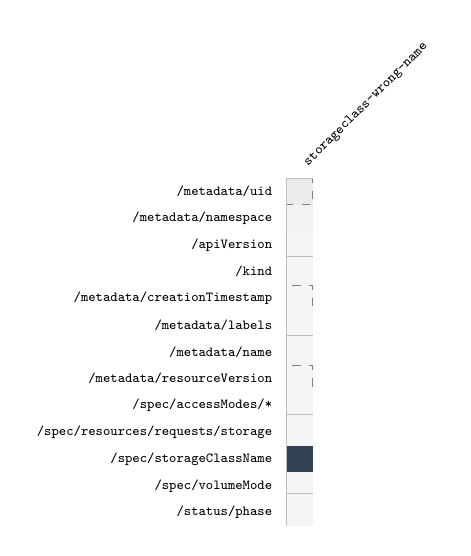
\begin{tikzpicture}[x=3.4mm,y=3.4mm]
\node[rotate=45,anchor=west,font=\ttfamily\tiny] at (0.5,0.25) {storageclass-wrong-name};
\node[anchor=east,font=\ttfamily\tiny] at (-0.15,-0.5) {/metadata/uid};
\fill[fill={rgb,255:red,235;green,236;blue,238}] (0,-1) rectangle ++(1,1);
\draw[gray,dashed,line width=0.2pt] (0,-1) rectangle ++(1,1);
\node[anchor=east,font=\ttfamily\tiny] at (-0.15,-1.5) {/metadata/namespace};
\fill[fill={rgb,255:red,241;green,242;blue,243}] (0,-2) rectangle ++(1,1);
\node[anchor=east,font=\ttfamily\tiny] at (-0.15,-2.5) {/apiVersion};
\fill[fill={rgb,255:red,244;green,244;blue,246}] (0,-3) rectangle ++(1,1);
\node[anchor=east,font=\ttfamily\tiny] at (-0.15,-3.5) {/kind};
\fill[fill={rgb,255:red,244;green,244;blue,246}] (0,-4) rectangle ++(1,1);
\node[anchor=east,font=\ttfamily\tiny] at (-0.15,-4.5) {/metadata/creationTimestamp};
\fill[fill={rgb,255:red,244;green,244;blue,246}] (0,-5) rectangle ++(1,1);
\draw[gray,dashed,line width=0.2pt] (0,-5) rectangle ++(1,1);
\node[anchor=east,font=\ttfamily\tiny] at (-0.15,-5.5) {/metadata/labels};
\fill[fill={rgb,255:red,244;green,244;blue,246}] (0,-6) rectangle ++(1,1);
\node[anchor=east,font=\ttfamily\tiny] at (-0.15,-6.5) {/metadata/name};
\fill[fill={rgb,255:red,244;green,244;blue,246}] (0,-7) rectangle ++(1,1);
\node[anchor=east,font=\ttfamily\tiny] at (-0.15,-7.5) {/metadata/resourceVersion};
\fill[fill={rgb,255:red,244;green,244;blue,246}] (0,-8) rectangle ++(1,1);
\draw[gray,dashed,line width=0.2pt] (0,-8) rectangle ++(1,1);
\node[anchor=east,font=\ttfamily\tiny] at (-0.15,-8.5) {/spec/accessModes/*};
\fill[fill={rgb,255:red,244;green,244;blue,246}] (0,-9) rectangle ++(1,1);
\node[anchor=east,font=\ttfamily\tiny] at (-0.15,-9.5) {/spec/resources/requests/storage};
\fill[fill={rgb,255:red,244;green,244;blue,246}] (0,-10) rectangle ++(1,1);
\node[anchor=east,font=\ttfamily\tiny] at (-0.15,-10.5) {/spec/storageClassName};
\fill[fill={rgb,255:red,51;green,65;blue,85}] (0,-11) rectangle ++(1,1);
\node[white,font=\tiny] at (0.5,-11.5) {$\ast$};
\node[anchor=east,font=\ttfamily\tiny] at (-0.15,-11.5) {/spec/volumeMode};
\fill[fill={rgb,255:red,244;green,244;blue,246}] (0,-12) rectangle ++(1,1);
\node[anchor=east,font=\ttfamily\tiny] at (-0.15,-12.5) {/status/phase};
\fill[fill={rgb,255:red,244;green,244;blue,246}] (0,-13) rectangle ++(1,1);
\draw[gray!50,line width=0.2pt] (0,0) grid (1,-13);
\end{tikzpicture}

\par\medskip\noindent{\small\bfseries ReplicaSet}\par\smallskip
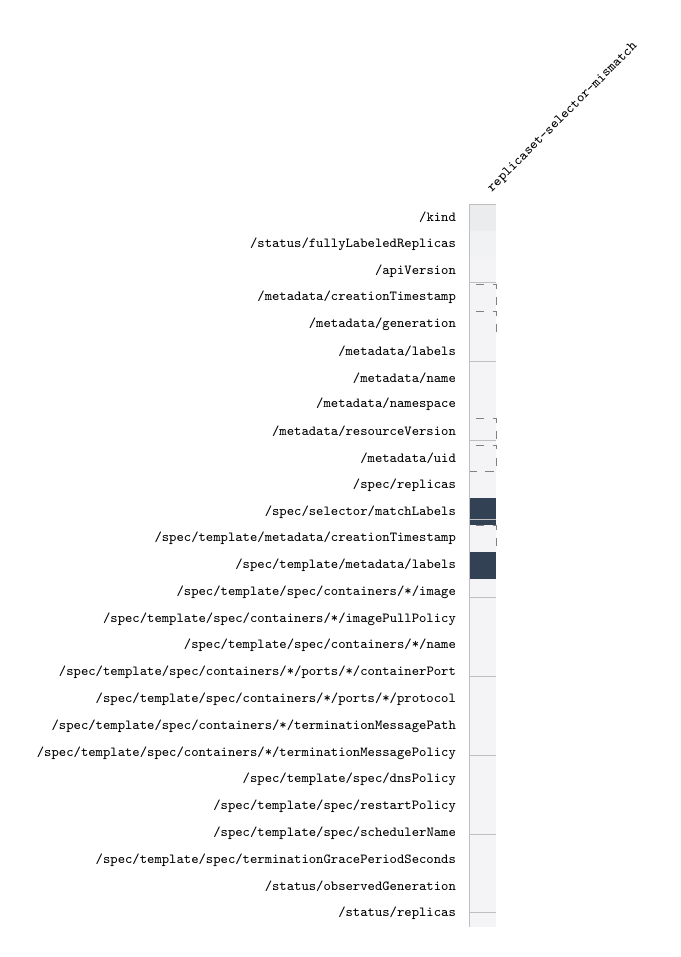
\begin{tikzpicture}[x=3.4mm,y=3.4mm]
\node[rotate=45,anchor=west,font=\ttfamily\tiny] at (0.5,0.25) {replicaset-selector-mismatch};
\node[anchor=east,font=\ttfamily\tiny] at (-0.15,-0.5) {/kind};
\fill[fill={rgb,255:red,235;green,236;blue,238}] (0,-1) rectangle ++(1,1);
\node[anchor=east,font=\ttfamily\tiny] at (-0.15,-1.5) {/status/fullyLabeledReplicas};
\fill[fill={rgb,255:red,241;green,242;blue,243}] (0,-2) rectangle ++(1,1);
\node[anchor=east,font=\ttfamily\tiny] at (-0.15,-2.5) {/apiVersion};
\fill[fill={rgb,255:red,244;green,244;blue,246}] (0,-3) rectangle ++(1,1);
\node[anchor=east,font=\ttfamily\tiny] at (-0.15,-3.5) {/metadata/creationTimestamp};
\fill[fill={rgb,255:red,244;green,244;blue,246}] (0,-4) rectangle ++(1,1);
\draw[gray,dashed,line width=0.2pt] (0,-4) rectangle ++(1,1);
\node[anchor=east,font=\ttfamily\tiny] at (-0.15,-4.5) {/metadata/generation};
\fill[fill={rgb,255:red,244;green,244;blue,246}] (0,-5) rectangle ++(1,1);
\draw[gray,dashed,line width=0.2pt] (0,-5) rectangle ++(1,1);
\node[anchor=east,font=\ttfamily\tiny] at (-0.15,-5.5) {/metadata/labels};
\fill[fill={rgb,255:red,244;green,244;blue,246}] (0,-6) rectangle ++(1,1);
\node[anchor=east,font=\ttfamily\tiny] at (-0.15,-6.5) {/metadata/name};
\fill[fill={rgb,255:red,244;green,244;blue,246}] (0,-7) rectangle ++(1,1);
\node[anchor=east,font=\ttfamily\tiny] at (-0.15,-7.5) {/metadata/namespace};
\fill[fill={rgb,255:red,244;green,244;blue,246}] (0,-8) rectangle ++(1,1);
\node[anchor=east,font=\ttfamily\tiny] at (-0.15,-8.5) {/metadata/resourceVersion};
\fill[fill={rgb,255:red,244;green,244;blue,246}] (0,-9) rectangle ++(1,1);
\draw[gray,dashed,line width=0.2pt] (0,-9) rectangle ++(1,1);
\node[anchor=east,font=\ttfamily\tiny] at (-0.15,-9.5) {/metadata/uid};
\fill[fill={rgb,255:red,244;green,244;blue,246}] (0,-10) rectangle ++(1,1);
\draw[gray,dashed,line width=0.2pt] (0,-10) rectangle ++(1,1);
\node[anchor=east,font=\ttfamily\tiny] at (-0.15,-10.5) {/spec/replicas};
\fill[fill={rgb,255:red,244;green,244;blue,246}] (0,-11) rectangle ++(1,1);
\node[anchor=east,font=\ttfamily\tiny] at (-0.15,-11.5) {/spec/selector/matchLabels};
\fill[fill={rgb,255:red,51;green,65;blue,85}] (0,-12) rectangle ++(1,1);
\node[white,font=\tiny] at (0.5,-12.5) {$\ast$};
\node[anchor=east,font=\ttfamily\tiny] at (-0.15,-12.5) {/spec/template/metadata/creationTimestamp};
\fill[fill={rgb,255:red,244;green,244;blue,246}] (0,-13) rectangle ++(1,1);
\draw[gray,dashed,line width=0.2pt] (0,-13) rectangle ++(1,1);
\node[anchor=east,font=\ttfamily\tiny] at (-0.15,-13.5) {/spec/template/metadata/labels};
\fill[fill={rgb,255:red,51;green,65;blue,85}] (0,-14) rectangle ++(1,1);
\node[white,font=\tiny] at (0.5,-14.5) {$\ast$};
\node[anchor=east,font=\ttfamily\tiny] at (-0.15,-14.5) {/spec/template/spec/containers/*/image};
\fill[fill={rgb,255:red,244;green,244;blue,246}] (0,-15) rectangle ++(1,1);
\node[anchor=east,font=\ttfamily\tiny] at (-0.15,-15.5) {/spec/template/spec/containers/*/imagePullPolicy};
\fill[fill={rgb,255:red,244;green,244;blue,246}] (0,-16) rectangle ++(1,1);
\node[anchor=east,font=\ttfamily\tiny] at (-0.15,-16.5) {/spec/template/spec/containers/*/name};
\fill[fill={rgb,255:red,244;green,244;blue,246}] (0,-17) rectangle ++(1,1);
\node[anchor=east,font=\ttfamily\tiny] at (-0.15,-17.5) {/spec/template/spec/containers/*/ports/*/containerPort};
\fill[fill={rgb,255:red,244;green,244;blue,246}] (0,-18) rectangle ++(1,1);
\node[anchor=east,font=\ttfamily\tiny] at (-0.15,-18.5) {/spec/template/spec/containers/*/ports/*/protocol};
\fill[fill={rgb,255:red,244;green,244;blue,246}] (0,-19) rectangle ++(1,1);
\node[anchor=east,font=\ttfamily\tiny] at (-0.15,-19.5) {/spec/template/spec/containers/*/terminationMessagePath};
\fill[fill={rgb,255:red,244;green,244;blue,246}] (0,-20) rectangle ++(1,1);
\node[anchor=east,font=\ttfamily\tiny] at (-0.15,-20.5) {/spec/template/spec/containers/*/terminationMessagePolicy};
\fill[fill={rgb,255:red,244;green,244;blue,246}] (0,-21) rectangle ++(1,1);
\node[anchor=east,font=\ttfamily\tiny] at (-0.15,-21.5) {/spec/template/spec/dnsPolicy};
\fill[fill={rgb,255:red,244;green,244;blue,246}] (0,-22) rectangle ++(1,1);
\node[anchor=east,font=\ttfamily\tiny] at (-0.15,-22.5) {/spec/template/spec/restartPolicy};
\fill[fill={rgb,255:red,244;green,244;blue,246}] (0,-23) rectangle ++(1,1);
\node[anchor=east,font=\ttfamily\tiny] at (-0.15,-23.5) {/spec/template/spec/schedulerName};
\fill[fill={rgb,255:red,244;green,244;blue,246}] (0,-24) rectangle ++(1,1);
\node[anchor=east,font=\ttfamily\tiny] at (-0.15,-24.5) {/spec/template/spec/terminationGracePeriodSeconds};
\fill[fill={rgb,255:red,244;green,244;blue,246}] (0,-25) rectangle ++(1,1);
\node[anchor=east,font=\ttfamily\tiny] at (-0.15,-25.5) {/status/observedGeneration};
\fill[fill={rgb,255:red,244;green,244;blue,246}] (0,-26) rectangle ++(1,1);
\node[anchor=east,font=\ttfamily\tiny] at (-0.15,-26.5) {/status/replicas};
\fill[fill={rgb,255:red,244;green,244;blue,246}] (0,-27) rectangle ++(1,1);
\draw[gray!50,line width=0.2pt] (0,0) grid (1,-27);
\end{tikzpicture}

\par\medskip\noindent{\small\bfseries StorageClass}\par\smallskip
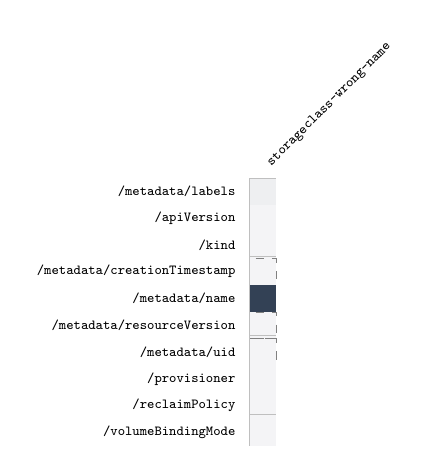
\begin{tikzpicture}[x=3.4mm,y=3.4mm]
\node[rotate=45,anchor=west,font=\ttfamily\tiny] at (0.5,0.25) {storageclass-wrong-name};
\node[anchor=east,font=\ttfamily\tiny] at (-0.15,-0.5) {/metadata/labels};
\fill[fill={rgb,255:red,238;green,239;blue,241}] (0,-1) rectangle ++(1,1);
\node[anchor=east,font=\ttfamily\tiny] at (-0.15,-1.5) {/apiVersion};
\fill[fill={rgb,255:red,244;green,244;blue,246}] (0,-2) rectangle ++(1,1);
\node[anchor=east,font=\ttfamily\tiny] at (-0.15,-2.5) {/kind};
\fill[fill={rgb,255:red,244;green,244;blue,246}] (0,-3) rectangle ++(1,1);
\node[anchor=east,font=\ttfamily\tiny] at (-0.15,-3.5) {/metadata/creationTimestamp};
\fill[fill={rgb,255:red,244;green,244;blue,246}] (0,-4) rectangle ++(1,1);
\draw[gray,dashed,line width=0.2pt] (0,-4) rectangle ++(1,1);
\node[anchor=east,font=\ttfamily\tiny] at (-0.15,-4.5) {/metadata/name};
\fill[fill={rgb,255:red,51;green,65;blue,85}] (0,-5) rectangle ++(1,1);
\node[white,font=\tiny] at (0.5,-5.5) {$\ast$};
\node[anchor=east,font=\ttfamily\tiny] at (-0.15,-5.5) {/metadata/resourceVersion};
\fill[fill={rgb,255:red,244;green,244;blue,246}] (0,-6) rectangle ++(1,1);
\draw[gray,dashed,line width=0.2pt] (0,-6) rectangle ++(1,1);
\node[anchor=east,font=\ttfamily\tiny] at (-0.15,-6.5) {/metadata/uid};
\fill[fill={rgb,255:red,244;green,244;blue,246}] (0,-7) rectangle ++(1,1);
\draw[gray,dashed,line width=0.2pt] (0,-7) rectangle ++(1,1);
\node[anchor=east,font=\ttfamily\tiny] at (-0.15,-7.5) {/provisioner};
\fill[fill={rgb,255:red,244;green,244;blue,246}] (0,-8) rectangle ++(1,1);
\node[anchor=east,font=\ttfamily\tiny] at (-0.15,-8.5) {/reclaimPolicy};
\fill[fill={rgb,255:red,244;green,244;blue,246}] (0,-9) rectangle ++(1,1);
\node[anchor=east,font=\ttfamily\tiny] at (-0.15,-9.5) {/volumeBindingMode};
\fill[fill={rgb,255:red,244;green,244;blue,246}] (0,-10) rectangle ++(1,1);
\draw[gray!50,line width=0.2pt] (0,0) grid (1,-10);
\end{tikzpicture}

\par\medskip\noindent{\small\bfseries Role}\par\smallskip
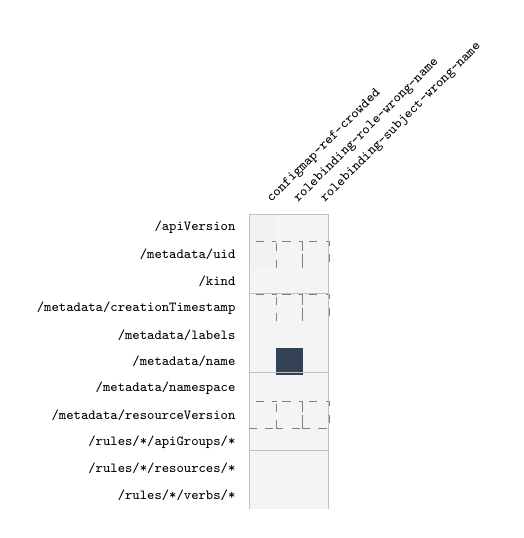
\begin{tikzpicture}[x=3.4mm,y=3.4mm]
\node[rotate=45,anchor=west,font=\ttfamily\tiny] at (0.5,0.25) {configmap-ref-crowded};
\node[rotate=45,anchor=west,font=\ttfamily\tiny] at (1.5,0.25) {rolebinding-role-wrong-name};
\node[rotate=45,anchor=west,font=\ttfamily\tiny] at (2.5,0.25) {rolebinding-subject-wrong-name};
\node[anchor=east,font=\ttfamily\tiny] at (-0.15,-0.5) {/apiVersion};
\fill[fill={rgb,255:red,241;green,242;blue,243}] (0,-1) rectangle ++(1,1);
\fill[fill={rgb,255:red,244;green,244;blue,246}] (1,-1) rectangle ++(1,1);
\fill[fill={rgb,255:red,244;green,244;blue,246}] (2,-1) rectangle ++(1,1);
\node[anchor=east,font=\ttfamily\tiny] at (-0.15,-1.5) {/metadata/uid};
\fill[fill={rgb,255:red,241;green,242;blue,243}] (0,-2) rectangle ++(1,1);
\draw[gray,dashed,line width=0.2pt] (0,-2) rectangle ++(1,1);
\fill[fill={rgb,255:red,244;green,244;blue,246}] (1,-2) rectangle ++(1,1);
\draw[gray,dashed,line width=0.2pt] (1,-2) rectangle ++(1,1);
\fill[fill={rgb,255:red,244;green,244;blue,246}] (2,-2) rectangle ++(1,1);
\draw[gray,dashed,line width=0.2pt] (2,-2) rectangle ++(1,1);
\node[anchor=east,font=\ttfamily\tiny] at (-0.15,-2.5) {/kind};
\fill[fill={rgb,255:red,244;green,244;blue,246}] (0,-3) rectangle ++(1,1);
\fill[fill={rgb,255:red,244;green,244;blue,246}] (1,-3) rectangle ++(1,1);
\fill[fill={rgb,255:red,244;green,244;blue,246}] (2,-3) rectangle ++(1,1);
\node[anchor=east,font=\ttfamily\tiny] at (-0.15,-3.5) {/metadata/creationTimestamp};
\fill[fill={rgb,255:red,244;green,244;blue,246}] (0,-4) rectangle ++(1,1);
\draw[gray,dashed,line width=0.2pt] (0,-4) rectangle ++(1,1);
\fill[fill={rgb,255:red,244;green,244;blue,246}] (1,-4) rectangle ++(1,1);
\draw[gray,dashed,line width=0.2pt] (1,-4) rectangle ++(1,1);
\fill[fill={rgb,255:red,244;green,244;blue,246}] (2,-4) rectangle ++(1,1);
\draw[gray,dashed,line width=0.2pt] (2,-4) rectangle ++(1,1);
\node[anchor=east,font=\ttfamily\tiny] at (-0.15,-4.5) {/metadata/labels};
\fill[fill={rgb,255:red,244;green,244;blue,246}] (0,-5) rectangle ++(1,1);
\fill[fill={rgb,255:red,244;green,244;blue,246}] (1,-5) rectangle ++(1,1);
\fill[fill={rgb,255:red,244;green,244;blue,246}] (2,-5) rectangle ++(1,1);
\node[anchor=east,font=\ttfamily\tiny] at (-0.15,-5.5) {/metadata/name};
\fill[fill={rgb,255:red,244;green,244;blue,246}] (0,-6) rectangle ++(1,1);
\fill[fill={rgb,255:red,51;green,65;blue,85}] (1,-6) rectangle ++(1,1);
\node[white,font=\tiny] at (1.5,-6.5) {$\ast$};
\fill[fill={rgb,255:red,244;green,244;blue,246}] (2,-6) rectangle ++(1,1);
\node[anchor=east,font=\ttfamily\tiny] at (-0.15,-6.5) {/metadata/namespace};
\fill[fill={rgb,255:red,244;green,244;blue,246}] (0,-7) rectangle ++(1,1);
\fill[fill={rgb,255:red,244;green,244;blue,246}] (1,-7) rectangle ++(1,1);
\fill[fill={rgb,255:red,244;green,244;blue,246}] (2,-7) rectangle ++(1,1);
\node[anchor=east,font=\ttfamily\tiny] at (-0.15,-7.5) {/metadata/resourceVersion};
\fill[fill={rgb,255:red,244;green,244;blue,246}] (0,-8) rectangle ++(1,1);
\draw[gray,dashed,line width=0.2pt] (0,-8) rectangle ++(1,1);
\fill[fill={rgb,255:red,244;green,244;blue,246}] (1,-8) rectangle ++(1,1);
\draw[gray,dashed,line width=0.2pt] (1,-8) rectangle ++(1,1);
\fill[fill={rgb,255:red,244;green,244;blue,246}] (2,-8) rectangle ++(1,1);
\draw[gray,dashed,line width=0.2pt] (2,-8) rectangle ++(1,1);
\node[anchor=east,font=\ttfamily\tiny] at (-0.15,-8.5) {/rules/*/apiGroups/*};
\fill[fill={rgb,255:red,244;green,244;blue,246}] (0,-9) rectangle ++(1,1);
\fill[fill={rgb,255:red,244;green,244;blue,246}] (1,-9) rectangle ++(1,1);
\fill[fill={rgb,255:red,244;green,244;blue,246}] (2,-9) rectangle ++(1,1);
\node[anchor=east,font=\ttfamily\tiny] at (-0.15,-9.5) {/rules/*/resources/*};
\fill[fill={rgb,255:red,244;green,244;blue,246}] (0,-10) rectangle ++(1,1);
\fill[fill={rgb,255:red,244;green,244;blue,246}] (1,-10) rectangle ++(1,1);
\fill[fill={rgb,255:red,244;green,244;blue,246}] (2,-10) rectangle ++(1,1);
\node[anchor=east,font=\ttfamily\tiny] at (-0.15,-10.5) {/rules/*/verbs/*};
\fill[fill={rgb,255:red,244;green,244;blue,246}] (0,-11) rectangle ++(1,1);
\fill[fill={rgb,255:red,244;green,244;blue,246}] (1,-11) rectangle ++(1,1);
\fill[fill={rgb,255:red,244;green,244;blue,246}] (2,-11) rectangle ++(1,1);
\draw[gray!50,line width=0.2pt] (0,0) grid (3,-11);
\end{tikzpicture}

\par\medskip\noindent{\small\bfseries RoleBinding}\par\smallskip
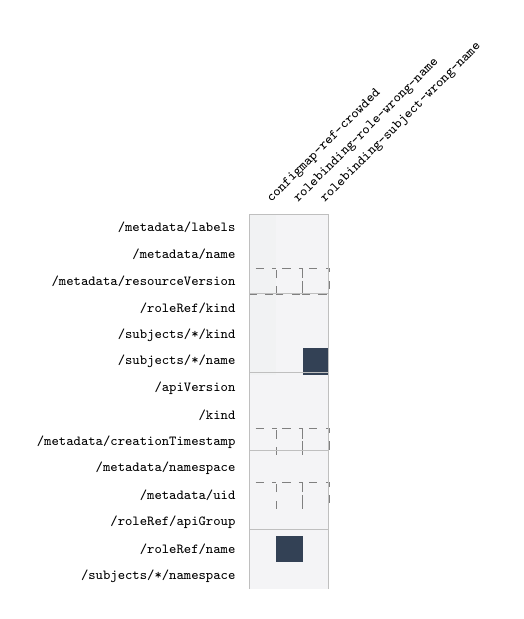
\begin{tikzpicture}[x=3.4mm,y=3.4mm]
\node[rotate=45,anchor=west,font=\ttfamily\tiny] at (0.5,0.25) {configmap-ref-crowded};
\node[rotate=45,anchor=west,font=\ttfamily\tiny] at (1.5,0.25) {rolebinding-role-wrong-name};
\node[rotate=45,anchor=west,font=\ttfamily\tiny] at (2.5,0.25) {rolebinding-subject-wrong-name};
\node[anchor=east,font=\ttfamily\tiny] at (-0.15,-0.5) {/metadata/labels};
\fill[fill={rgb,255:red,241;green,242;blue,243}] (0,-1) rectangle ++(1,1);
\fill[fill={rgb,255:red,244;green,244;blue,246}] (1,-1) rectangle ++(1,1);
\fill[fill={rgb,255:red,244;green,244;blue,246}] (2,-1) rectangle ++(1,1);
\node[anchor=east,font=\ttfamily\tiny] at (-0.15,-1.5) {/metadata/name};
\fill[fill={rgb,255:red,241;green,242;blue,243}] (0,-2) rectangle ++(1,1);
\fill[fill={rgb,255:red,244;green,244;blue,246}] (1,-2) rectangle ++(1,1);
\fill[fill={rgb,255:red,244;green,244;blue,246}] (2,-2) rectangle ++(1,1);
\node[anchor=east,font=\ttfamily\tiny] at (-0.15,-2.5) {/metadata/resourceVersion};
\fill[fill={rgb,255:red,241;green,242;blue,243}] (0,-3) rectangle ++(1,1);
\draw[gray,dashed,line width=0.2pt] (0,-3) rectangle ++(1,1);
\fill[fill={rgb,255:red,244;green,244;blue,246}] (1,-3) rectangle ++(1,1);
\draw[gray,dashed,line width=0.2pt] (1,-3) rectangle ++(1,1);
\fill[fill={rgb,255:red,244;green,244;blue,246}] (2,-3) rectangle ++(1,1);
\draw[gray,dashed,line width=0.2pt] (2,-3) rectangle ++(1,1);
\node[anchor=east,font=\ttfamily\tiny] at (-0.15,-3.5) {/roleRef/kind};
\fill[fill={rgb,255:red,241;green,242;blue,243}] (0,-4) rectangle ++(1,1);
\fill[fill={rgb,255:red,244;green,244;blue,246}] (1,-4) rectangle ++(1,1);
\fill[fill={rgb,255:red,244;green,244;blue,246}] (2,-4) rectangle ++(1,1);
\node[anchor=east,font=\ttfamily\tiny] at (-0.15,-4.5) {/subjects/*/kind};
\fill[fill={rgb,255:red,241;green,242;blue,243}] (0,-5) rectangle ++(1,1);
\fill[fill={rgb,255:red,244;green,244;blue,246}] (1,-5) rectangle ++(1,1);
\fill[fill={rgb,255:red,244;green,244;blue,246}] (2,-5) rectangle ++(1,1);
\node[anchor=east,font=\ttfamily\tiny] at (-0.15,-5.5) {/subjects/*/name};
\fill[fill={rgb,255:red,241;green,242;blue,243}] (0,-6) rectangle ++(1,1);
\fill[fill={rgb,255:red,244;green,244;blue,246}] (1,-6) rectangle ++(1,1);
\fill[fill={rgb,255:red,51;green,65;blue,85}] (2,-6) rectangle ++(1,1);
\node[white,font=\tiny] at (2.5,-6.5) {$\ast$};
\node[anchor=east,font=\ttfamily\tiny] at (-0.15,-6.5) {/apiVersion};
\fill[fill={rgb,255:red,244;green,244;blue,246}] (0,-7) rectangle ++(1,1);
\fill[fill={rgb,255:red,244;green,244;blue,246}] (1,-7) rectangle ++(1,1);
\fill[fill={rgb,255:red,244;green,244;blue,246}] (2,-7) rectangle ++(1,1);
\node[anchor=east,font=\ttfamily\tiny] at (-0.15,-7.5) {/kind};
\fill[fill={rgb,255:red,244;green,244;blue,246}] (0,-8) rectangle ++(1,1);
\fill[fill={rgb,255:red,244;green,244;blue,246}] (1,-8) rectangle ++(1,1);
\fill[fill={rgb,255:red,244;green,244;blue,246}] (2,-8) rectangle ++(1,1);
\node[anchor=east,font=\ttfamily\tiny] at (-0.15,-8.5) {/metadata/creationTimestamp};
\fill[fill={rgb,255:red,244;green,244;blue,246}] (0,-9) rectangle ++(1,1);
\draw[gray,dashed,line width=0.2pt] (0,-9) rectangle ++(1,1);
\fill[fill={rgb,255:red,244;green,244;blue,246}] (1,-9) rectangle ++(1,1);
\draw[gray,dashed,line width=0.2pt] (1,-9) rectangle ++(1,1);
\fill[fill={rgb,255:red,244;green,244;blue,246}] (2,-9) rectangle ++(1,1);
\draw[gray,dashed,line width=0.2pt] (2,-9) rectangle ++(1,1);
\node[anchor=east,font=\ttfamily\tiny] at (-0.15,-9.5) {/metadata/namespace};
\fill[fill={rgb,255:red,244;green,244;blue,246}] (0,-10) rectangle ++(1,1);
\fill[fill={rgb,255:red,244;green,244;blue,246}] (1,-10) rectangle ++(1,1);
\fill[fill={rgb,255:red,244;green,244;blue,246}] (2,-10) rectangle ++(1,1);
\node[anchor=east,font=\ttfamily\tiny] at (-0.15,-10.5) {/metadata/uid};
\fill[fill={rgb,255:red,244;green,244;blue,246}] (0,-11) rectangle ++(1,1);
\draw[gray,dashed,line width=0.2pt] (0,-11) rectangle ++(1,1);
\fill[fill={rgb,255:red,244;green,244;blue,246}] (1,-11) rectangle ++(1,1);
\draw[gray,dashed,line width=0.2pt] (1,-11) rectangle ++(1,1);
\fill[fill={rgb,255:red,244;green,244;blue,246}] (2,-11) rectangle ++(1,1);
\draw[gray,dashed,line width=0.2pt] (2,-11) rectangle ++(1,1);
\node[anchor=east,font=\ttfamily\tiny] at (-0.15,-11.5) {/roleRef/apiGroup};
\fill[fill={rgb,255:red,244;green,244;blue,246}] (0,-12) rectangle ++(1,1);
\fill[fill={rgb,255:red,244;green,244;blue,246}] (1,-12) rectangle ++(1,1);
\fill[fill={rgb,255:red,244;green,244;blue,246}] (2,-12) rectangle ++(1,1);
\node[anchor=east,font=\ttfamily\tiny] at (-0.15,-12.5) {/roleRef/name};
\fill[fill={rgb,255:red,244;green,244;blue,246}] (0,-13) rectangle ++(1,1);
\fill[fill={rgb,255:red,51;green,65;blue,85}] (1,-13) rectangle ++(1,1);
\node[white,font=\tiny] at (1.5,-13.5) {$\ast$};
\fill[fill={rgb,255:red,244;green,244;blue,246}] (2,-13) rectangle ++(1,1);
\node[anchor=east,font=\ttfamily\tiny] at (-0.15,-13.5) {/subjects/*/namespace};
\fill[fill={rgb,255:red,244;green,244;blue,246}] (0,-14) rectangle ++(1,1);
\fill[fill={rgb,255:red,244;green,244;blue,246}] (1,-14) rectangle ++(1,1);
\fill[fill={rgb,255:red,244;green,244;blue,246}] (2,-14) rectangle ++(1,1);
\draw[gray!50,line width=0.2pt] (0,0) grid (3,-14);
\end{tikzpicture}

\par\medskip\noindent{\small\bfseries Ingress}\par\smallskip
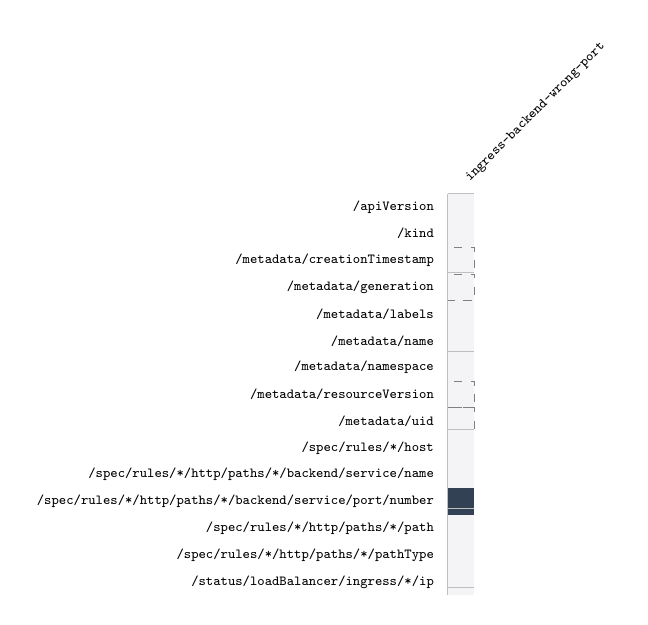
\begin{tikzpicture}[x=3.4mm,y=3.4mm]
\node[rotate=45,anchor=west,font=\ttfamily\tiny] at (0.5,0.25) {ingress-backend-wrong-port};
\node[anchor=east,font=\ttfamily\tiny] at (-0.15,-0.5) {/apiVersion};
\fill[fill={rgb,255:red,244;green,244;blue,246}] (0,-1) rectangle ++(1,1);
\node[anchor=east,font=\ttfamily\tiny] at (-0.15,-1.5) {/kind};
\fill[fill={rgb,255:red,244;green,244;blue,246}] (0,-2) rectangle ++(1,1);
\node[anchor=east,font=\ttfamily\tiny] at (-0.15,-2.5) {/metadata/creationTimestamp};
\fill[fill={rgb,255:red,244;green,244;blue,246}] (0,-3) rectangle ++(1,1);
\draw[gray,dashed,line width=0.2pt] (0,-3) rectangle ++(1,1);
\node[anchor=east,font=\ttfamily\tiny] at (-0.15,-3.5) {/metadata/generation};
\fill[fill={rgb,255:red,244;green,244;blue,246}] (0,-4) rectangle ++(1,1);
\draw[gray,dashed,line width=0.2pt] (0,-4) rectangle ++(1,1);
\node[anchor=east,font=\ttfamily\tiny] at (-0.15,-4.5) {/metadata/labels};
\fill[fill={rgb,255:red,244;green,244;blue,246}] (0,-5) rectangle ++(1,1);
\node[anchor=east,font=\ttfamily\tiny] at (-0.15,-5.5) {/metadata/name};
\fill[fill={rgb,255:red,244;green,244;blue,246}] (0,-6) rectangle ++(1,1);
\node[anchor=east,font=\ttfamily\tiny] at (-0.15,-6.5) {/metadata/namespace};
\fill[fill={rgb,255:red,244;green,244;blue,246}] (0,-7) rectangle ++(1,1);
\node[anchor=east,font=\ttfamily\tiny] at (-0.15,-7.5) {/metadata/resourceVersion};
\fill[fill={rgb,255:red,244;green,244;blue,246}] (0,-8) rectangle ++(1,1);
\draw[gray,dashed,line width=0.2pt] (0,-8) rectangle ++(1,1);
\node[anchor=east,font=\ttfamily\tiny] at (-0.15,-8.5) {/metadata/uid};
\fill[fill={rgb,255:red,244;green,244;blue,246}] (0,-9) rectangle ++(1,1);
\draw[gray,dashed,line width=0.2pt] (0,-9) rectangle ++(1,1);
\node[anchor=east,font=\ttfamily\tiny] at (-0.15,-9.5) {/spec/rules/*/host};
\fill[fill={rgb,255:red,244;green,244;blue,246}] (0,-10) rectangle ++(1,1);
\node[anchor=east,font=\ttfamily\tiny] at (-0.15,-10.5) {/spec/rules/*/http/paths/*/backend/service/name};
\fill[fill={rgb,255:red,244;green,244;blue,246}] (0,-11) rectangle ++(1,1);
\node[anchor=east,font=\ttfamily\tiny] at (-0.15,-11.5) {/spec/rules/*/http/paths/*/backend/service/port/number};
\fill[fill={rgb,255:red,51;green,65;blue,85}] (0,-12) rectangle ++(1,1);
\node[white,font=\tiny] at (0.5,-12.5) {$\ast$};
\node[anchor=east,font=\ttfamily\tiny] at (-0.15,-12.5) {/spec/rules/*/http/paths/*/path};
\fill[fill={rgb,255:red,244;green,244;blue,246}] (0,-13) rectangle ++(1,1);
\node[anchor=east,font=\ttfamily\tiny] at (-0.15,-13.5) {/spec/rules/*/http/paths/*/pathType};
\fill[fill={rgb,255:red,244;green,244;blue,246}] (0,-14) rectangle ++(1,1);
\node[anchor=east,font=\ttfamily\tiny] at (-0.15,-14.5) {/status/loadBalancer/ingress/*/ip};
\fill[fill={rgb,255:red,244;green,244;blue,246}] (0,-15) rectangle ++(1,1);
\draw[gray!50,line width=0.2pt] (0,0) grid (1,-15);
\end{tikzpicture}

\par\medskip\noindent{\small\bfseries Secret}\par\smallskip
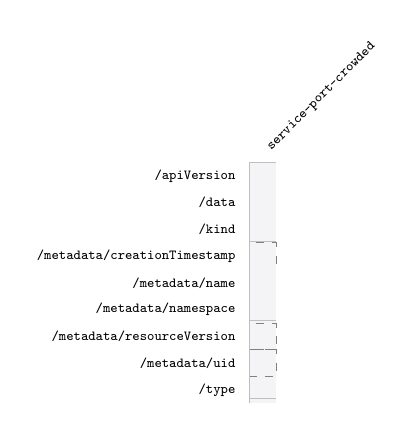
\begin{tikzpicture}[x=3.4mm,y=3.4mm]
\node[rotate=45,anchor=west,font=\ttfamily\tiny] at (0.5,0.25) {service-port-crowded};
\node[anchor=east,font=\ttfamily\tiny] at (-0.15,-0.5) {/apiVersion};
\fill[fill={rgb,255:red,244;green,244;blue,246}] (0,-1) rectangle ++(1,1);
\node[anchor=east,font=\ttfamily\tiny] at (-0.15,-1.5) {/data};
\fill[fill={rgb,255:red,244;green,244;blue,246}] (0,-2) rectangle ++(1,1);
\node[anchor=east,font=\ttfamily\tiny] at (-0.15,-2.5) {/kind};
\fill[fill={rgb,255:red,244;green,244;blue,246}] (0,-3) rectangle ++(1,1);
\node[anchor=east,font=\ttfamily\tiny] at (-0.15,-3.5) {/metadata/creationTimestamp};
\fill[fill={rgb,255:red,244;green,244;blue,246}] (0,-4) rectangle ++(1,1);
\draw[gray,dashed,line width=0.2pt] (0,-4) rectangle ++(1,1);
\node[anchor=east,font=\ttfamily\tiny] at (-0.15,-4.5) {/metadata/name};
\fill[fill={rgb,255:red,244;green,244;blue,246}] (0,-5) rectangle ++(1,1);
\node[anchor=east,font=\ttfamily\tiny] at (-0.15,-5.5) {/metadata/namespace};
\fill[fill={rgb,255:red,244;green,244;blue,246}] (0,-6) rectangle ++(1,1);
\node[anchor=east,font=\ttfamily\tiny] at (-0.15,-6.5) {/metadata/resourceVersion};
\fill[fill={rgb,255:red,244;green,244;blue,246}] (0,-7) rectangle ++(1,1);
\draw[gray,dashed,line width=0.2pt] (0,-7) rectangle ++(1,1);
\node[anchor=east,font=\ttfamily\tiny] at (-0.15,-7.5) {/metadata/uid};
\fill[fill={rgb,255:red,244;green,244;blue,246}] (0,-8) rectangle ++(1,1);
\draw[gray,dashed,line width=0.2pt] (0,-8) rectangle ++(1,1);
\node[anchor=east,font=\ttfamily\tiny] at (-0.15,-8.5) {/type};
\fill[fill={rgb,255:red,244;green,244;blue,246}] (0,-9) rectangle ++(1,1);
\draw[gray!50,line width=0.2pt] (0,0) grid (1,-9);
\end{tikzpicture}

\par\medskip\noindent{\small\bfseries StatefulSet}\par\smallskip
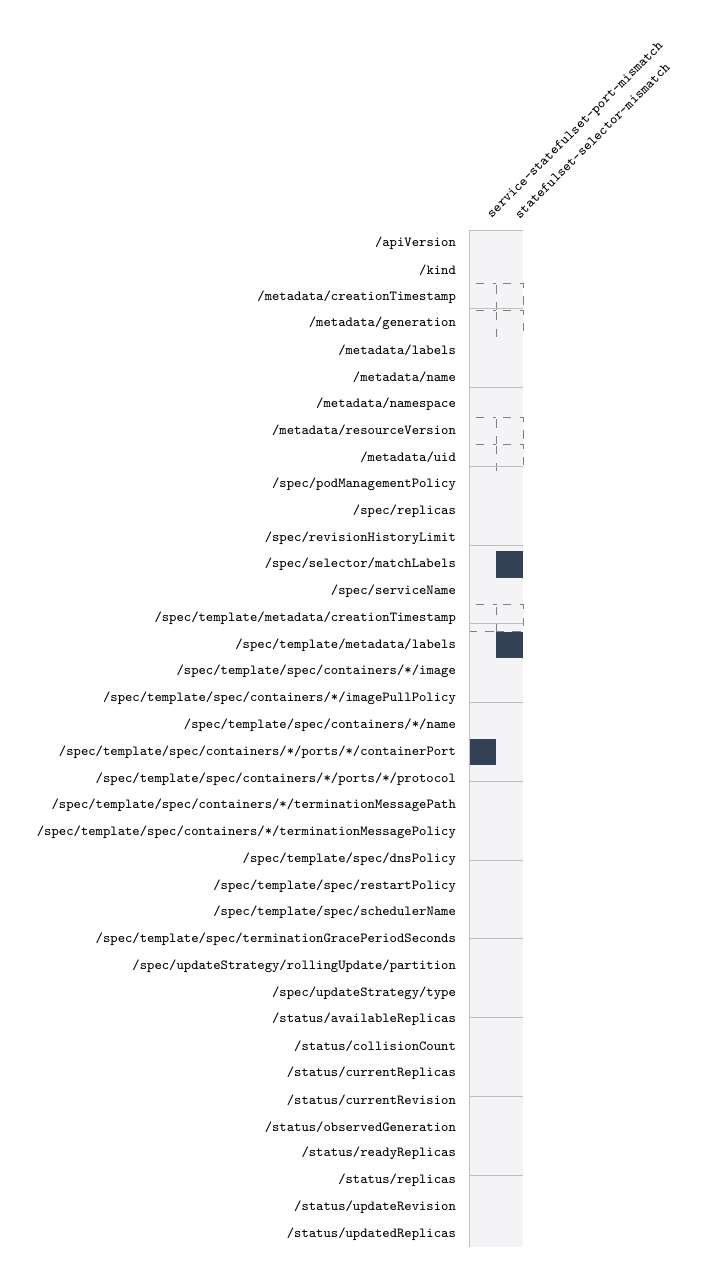
\begin{tikzpicture}[x=3.4mm,y=3.4mm]
\node[rotate=45,anchor=west,font=\ttfamily\tiny] at (0.5,0.25) {service-statefulset-port-mismatch};
\node[rotate=45,anchor=west,font=\ttfamily\tiny] at (1.5,0.25) {statefulset-selector-mismatch};
\node[anchor=east,font=\ttfamily\tiny] at (-0.15,-0.5) {/apiVersion};
\fill[fill={rgb,255:red,244;green,244;blue,246}] (0,-1) rectangle ++(1,1);
\fill[fill={rgb,255:red,244;green,244;blue,246}] (1,-1) rectangle ++(1,1);
\node[anchor=east,font=\ttfamily\tiny] at (-0.15,-1.5) {/kind};
\fill[fill={rgb,255:red,244;green,244;blue,246}] (0,-2) rectangle ++(1,1);
\fill[fill={rgb,255:red,244;green,244;blue,246}] (1,-2) rectangle ++(1,1);
\node[anchor=east,font=\ttfamily\tiny] at (-0.15,-2.5) {/metadata/creationTimestamp};
\fill[fill={rgb,255:red,244;green,244;blue,246}] (0,-3) rectangle ++(1,1);
\draw[gray,dashed,line width=0.2pt] (0,-3) rectangle ++(1,1);
\fill[fill={rgb,255:red,244;green,244;blue,246}] (1,-3) rectangle ++(1,1);
\draw[gray,dashed,line width=0.2pt] (1,-3) rectangle ++(1,1);
\node[anchor=east,font=\ttfamily\tiny] at (-0.15,-3.5) {/metadata/generation};
\fill[fill={rgb,255:red,244;green,244;blue,246}] (0,-4) rectangle ++(1,1);
\draw[gray,dashed,line width=0.2pt] (0,-4) rectangle ++(1,1);
\fill[fill={rgb,255:red,244;green,244;blue,246}] (1,-4) rectangle ++(1,1);
\draw[gray,dashed,line width=0.2pt] (1,-4) rectangle ++(1,1);
\node[anchor=east,font=\ttfamily\tiny] at (-0.15,-4.5) {/metadata/labels};
\fill[fill={rgb,255:red,244;green,244;blue,246}] (0,-5) rectangle ++(1,1);
\fill[fill={rgb,255:red,244;green,244;blue,246}] (1,-5) rectangle ++(1,1);
\node[anchor=east,font=\ttfamily\tiny] at (-0.15,-5.5) {/metadata/name};
\fill[fill={rgb,255:red,244;green,244;blue,246}] (0,-6) rectangle ++(1,1);
\fill[fill={rgb,255:red,244;green,244;blue,246}] (1,-6) rectangle ++(1,1);
\node[anchor=east,font=\ttfamily\tiny] at (-0.15,-6.5) {/metadata/namespace};
\fill[fill={rgb,255:red,244;green,244;blue,246}] (0,-7) rectangle ++(1,1);
\fill[fill={rgb,255:red,244;green,244;blue,246}] (1,-7) rectangle ++(1,1);
\node[anchor=east,font=\ttfamily\tiny] at (-0.15,-7.5) {/metadata/resourceVersion};
\fill[fill={rgb,255:red,244;green,244;blue,246}] (0,-8) rectangle ++(1,1);
\draw[gray,dashed,line width=0.2pt] (0,-8) rectangle ++(1,1);
\fill[fill={rgb,255:red,244;green,244;blue,246}] (1,-8) rectangle ++(1,1);
\draw[gray,dashed,line width=0.2pt] (1,-8) rectangle ++(1,1);
\node[anchor=east,font=\ttfamily\tiny] at (-0.15,-8.5) {/metadata/uid};
\fill[fill={rgb,255:red,244;green,244;blue,246}] (0,-9) rectangle ++(1,1);
\draw[gray,dashed,line width=0.2pt] (0,-9) rectangle ++(1,1);
\fill[fill={rgb,255:red,244;green,244;blue,246}] (1,-9) rectangle ++(1,1);
\draw[gray,dashed,line width=0.2pt] (1,-9) rectangle ++(1,1);
\node[anchor=east,font=\ttfamily\tiny] at (-0.15,-9.5) {/spec/podManagementPolicy};
\fill[fill={rgb,255:red,244;green,244;blue,246}] (0,-10) rectangle ++(1,1);
\fill[fill={rgb,255:red,244;green,244;blue,246}] (1,-10) rectangle ++(1,1);
\node[anchor=east,font=\ttfamily\tiny] at (-0.15,-10.5) {/spec/replicas};
\fill[fill={rgb,255:red,244;green,244;blue,246}] (0,-11) rectangle ++(1,1);
\fill[fill={rgb,255:red,244;green,244;blue,246}] (1,-11) rectangle ++(1,1);
\node[anchor=east,font=\ttfamily\tiny] at (-0.15,-11.5) {/spec/revisionHistoryLimit};
\fill[fill={rgb,255:red,244;green,244;blue,246}] (0,-12) rectangle ++(1,1);
\fill[fill={rgb,255:red,244;green,244;blue,246}] (1,-12) rectangle ++(1,1);
\node[anchor=east,font=\ttfamily\tiny] at (-0.15,-12.5) {/spec/selector/matchLabels};
\fill[fill={rgb,255:red,244;green,244;blue,246}] (0,-13) rectangle ++(1,1);
\fill[fill={rgb,255:red,51;green,65;blue,85}] (1,-13) rectangle ++(1,1);
\node[white,font=\tiny] at (1.5,-13.5) {$\ast$};
\node[anchor=east,font=\ttfamily\tiny] at (-0.15,-13.5) {/spec/serviceName};
\fill[fill={rgb,255:red,244;green,244;blue,246}] (0,-14) rectangle ++(1,1);
\fill[fill={rgb,255:red,244;green,244;blue,246}] (1,-14) rectangle ++(1,1);
\node[anchor=east,font=\ttfamily\tiny] at (-0.15,-14.5) {/spec/template/metadata/creationTimestamp};
\fill[fill={rgb,255:red,244;green,244;blue,246}] (0,-15) rectangle ++(1,1);
\draw[gray,dashed,line width=0.2pt] (0,-15) rectangle ++(1,1);
\fill[fill={rgb,255:red,244;green,244;blue,246}] (1,-15) rectangle ++(1,1);
\draw[gray,dashed,line width=0.2pt] (1,-15) rectangle ++(1,1);
\node[anchor=east,font=\ttfamily\tiny] at (-0.15,-15.5) {/spec/template/metadata/labels};
\fill[fill={rgb,255:red,244;green,244;blue,246}] (0,-16) rectangle ++(1,1);
\fill[fill={rgb,255:red,51;green,65;blue,85}] (1,-16) rectangle ++(1,1);
\node[white,font=\tiny] at (1.5,-16.5) {$\ast$};
\node[anchor=east,font=\ttfamily\tiny] at (-0.15,-16.5) {/spec/template/spec/containers/*/image};
\fill[fill={rgb,255:red,244;green,244;blue,246}] (0,-17) rectangle ++(1,1);
\fill[fill={rgb,255:red,244;green,244;blue,246}] (1,-17) rectangle ++(1,1);
\node[anchor=east,font=\ttfamily\tiny] at (-0.15,-17.5) {/spec/template/spec/containers/*/imagePullPolicy};
\fill[fill={rgb,255:red,244;green,244;blue,246}] (0,-18) rectangle ++(1,1);
\fill[fill={rgb,255:red,244;green,244;blue,246}] (1,-18) rectangle ++(1,1);
\node[anchor=east,font=\ttfamily\tiny] at (-0.15,-18.5) {/spec/template/spec/containers/*/name};
\fill[fill={rgb,255:red,244;green,244;blue,246}] (0,-19) rectangle ++(1,1);
\fill[fill={rgb,255:red,244;green,244;blue,246}] (1,-19) rectangle ++(1,1);
\node[anchor=east,font=\ttfamily\tiny] at (-0.15,-19.5) {/spec/template/spec/containers/*/ports/*/containerPort};
\fill[fill={rgb,255:red,51;green,65;blue,85}] (0,-20) rectangle ++(1,1);
\node[white,font=\tiny] at (0.5,-20.5) {$\ast$};
\fill[fill={rgb,255:red,244;green,244;blue,246}] (1,-20) rectangle ++(1,1);
\node[anchor=east,font=\ttfamily\tiny] at (-0.15,-20.5) {/spec/template/spec/containers/*/ports/*/protocol};
\fill[fill={rgb,255:red,244;green,244;blue,246}] (0,-21) rectangle ++(1,1);
\fill[fill={rgb,255:red,244;green,244;blue,246}] (1,-21) rectangle ++(1,1);
\node[anchor=east,font=\ttfamily\tiny] at (-0.15,-21.5) {/spec/template/spec/containers/*/terminationMessagePath};
\fill[fill={rgb,255:red,244;green,244;blue,246}] (0,-22) rectangle ++(1,1);
\fill[fill={rgb,255:red,244;green,244;blue,246}] (1,-22) rectangle ++(1,1);
\node[anchor=east,font=\ttfamily\tiny] at (-0.15,-22.5) {/spec/template/spec/containers/*/terminationMessagePolicy};
\fill[fill={rgb,255:red,244;green,244;blue,246}] (0,-23) rectangle ++(1,1);
\fill[fill={rgb,255:red,244;green,244;blue,246}] (1,-23) rectangle ++(1,1);
\node[anchor=east,font=\ttfamily\tiny] at (-0.15,-23.5) {/spec/template/spec/dnsPolicy};
\fill[fill={rgb,255:red,244;green,244;blue,246}] (0,-24) rectangle ++(1,1);
\fill[fill={rgb,255:red,244;green,244;blue,246}] (1,-24) rectangle ++(1,1);
\node[anchor=east,font=\ttfamily\tiny] at (-0.15,-24.5) {/spec/template/spec/restartPolicy};
\fill[fill={rgb,255:red,244;green,244;blue,246}] (0,-25) rectangle ++(1,1);
\fill[fill={rgb,255:red,244;green,244;blue,246}] (1,-25) rectangle ++(1,1);
\node[anchor=east,font=\ttfamily\tiny] at (-0.15,-25.5) {/spec/template/spec/schedulerName};
\fill[fill={rgb,255:red,244;green,244;blue,246}] (0,-26) rectangle ++(1,1);
\fill[fill={rgb,255:red,244;green,244;blue,246}] (1,-26) rectangle ++(1,1);
\node[anchor=east,font=\ttfamily\tiny] at (-0.15,-26.5) {/spec/template/spec/terminationGracePeriodSeconds};
\fill[fill={rgb,255:red,244;green,244;blue,246}] (0,-27) rectangle ++(1,1);
\fill[fill={rgb,255:red,244;green,244;blue,246}] (1,-27) rectangle ++(1,1);
\node[anchor=east,font=\ttfamily\tiny] at (-0.15,-27.5) {/spec/updateStrategy/rollingUpdate/partition};
\fill[fill={rgb,255:red,244;green,244;blue,246}] (0,-28) rectangle ++(1,1);
\fill[fill={rgb,255:red,244;green,244;blue,246}] (1,-28) rectangle ++(1,1);
\node[anchor=east,font=\ttfamily\tiny] at (-0.15,-28.5) {/spec/updateStrategy/type};
\fill[fill={rgb,255:red,244;green,244;blue,246}] (0,-29) rectangle ++(1,1);
\fill[fill={rgb,255:red,244;green,244;blue,246}] (1,-29) rectangle ++(1,1);
\node[anchor=east,font=\ttfamily\tiny] at (-0.15,-29.5) {/status/availableReplicas};
\fill[fill={rgb,255:red,244;green,244;blue,246}] (0,-30) rectangle ++(1,1);
\fill[fill={rgb,255:red,244;green,244;blue,246}] (1,-30) rectangle ++(1,1);
\node[anchor=east,font=\ttfamily\tiny] at (-0.15,-30.5) {/status/collisionCount};
\fill[fill={rgb,255:red,244;green,244;blue,246}] (0,-31) rectangle ++(1,1);
\fill[fill={rgb,255:red,244;green,244;blue,246}] (1,-31) rectangle ++(1,1);
\node[anchor=east,font=\ttfamily\tiny] at (-0.15,-31.5) {/status/currentReplicas};
\fill[fill={rgb,255:red,244;green,244;blue,246}] (0,-32) rectangle ++(1,1);
\fill[fill={rgb,255:red,244;green,244;blue,246}] (1,-32) rectangle ++(1,1);
\node[anchor=east,font=\ttfamily\tiny] at (-0.15,-32.5) {/status/currentRevision};
\fill[fill={rgb,255:red,244;green,244;blue,246}] (0,-33) rectangle ++(1,1);
\fill[fill={rgb,255:red,244;green,244;blue,246}] (1,-33) rectangle ++(1,1);
\node[anchor=east,font=\ttfamily\tiny] at (-0.15,-33.5) {/status/observedGeneration};
\fill[fill={rgb,255:red,244;green,244;blue,246}] (0,-34) rectangle ++(1,1);
\fill[fill={rgb,255:red,244;green,244;blue,246}] (1,-34) rectangle ++(1,1);
\node[anchor=east,font=\ttfamily\tiny] at (-0.15,-34.5) {/status/readyReplicas};
\fill[fill={rgb,255:red,244;green,244;blue,246}] (0,-35) rectangle ++(1,1);
\fill[fill={rgb,255:red,244;green,244;blue,246}] (1,-35) rectangle ++(1,1);
\node[anchor=east,font=\ttfamily\tiny] at (-0.15,-35.5) {/status/replicas};
\fill[fill={rgb,255:red,244;green,244;blue,246}] (0,-36) rectangle ++(1,1);
\fill[fill={rgb,255:red,244;green,244;blue,246}] (1,-36) rectangle ++(1,1);
\node[anchor=east,font=\ttfamily\tiny] at (-0.15,-36.5) {/status/updateRevision};
\fill[fill={rgb,255:red,244;green,244;blue,246}] (0,-37) rectangle ++(1,1);
\fill[fill={rgb,255:red,244;green,244;blue,246}] (1,-37) rectangle ++(1,1);
\node[anchor=east,font=\ttfamily\tiny] at (-0.15,-37.5) {/status/updatedReplicas};
\fill[fill={rgb,255:red,244;green,244;blue,246}] (0,-38) rectangle ++(1,1);
\fill[fill={rgb,255:red,244;green,244;blue,246}] (1,-38) rectangle ++(1,1);
\draw[gray!50,line width=0.2pt] (0,0) grid (2,-38);
\end{tikzpicture}
